% $Id: tutorialAndQuickStartGuide.tex,v 4.19 2008/12/17 00:55:44 alglomana Exp $
\documentclass[a4paper, 11pt]{article}
\marginparwidth 0pt
\oddsidemargin  0pt
\evensidemargin  0pt
\marginparsep 0pt
\topmargin   0pt
\textwidth   6.5in
\textheight  8.5 in
\usepackage{graphicx}
\usepackage{natbib}
\usepackage{fancyvrb}
\usepackage{lscape}
\usepackage{url}
\usepackage{hyperref}
\setcounter{secnumdepth}{5}
\setcounter{tocdepth}{5}
\hypersetup{
  colorlinks,
  citecolor=cyan,
  filecolor=blue,
  linkcolor=blue,
  urlcolor=magenta
}
\begin{document}
  \begin{center}
    \thispagestyle{empty}
    \textbf{\Large{\texttt{ByoDyn} Tutorial and Quick Start Guide for \texttt{ByoDyn} version 4.8}}\\[5ex]
    \textbf{Adri\'an L\'opez Garc\'ia de Lomana, Alex G\'omez-Garrido, Miguel Hern\'andez, Pau Ru\'e Queralt and Jordi Vill\`a-Freixa}\\[10ex] --- December 17, 2008 ---\\[10ex]
    \parbox{0.70\linewidth}{
      This document gives short description about the functionalities of \texttt{ByoDyn} as a quick start guide. 
      On the tutorial we will show a set of examples on the use of \texttt{ByoDyn} for the study of a dynamic system.
      From a computational point of view we describe and analyze here a bunch of relevant biochemical systems.
      We give examples about metabolic networks, engineered gene networks and multicellular pattern formation.
      All the examples will be illustrated with the help of the computational tool \texttt{ByoDyn}.
    }\\[40ex]
  \end{center}
  \begin{footnotesize}
    \begin{raggedleft}
      \textbf{Computational Biochemistry and Biophysics Laboratory}\\
      Research Unit on Biomedical Informatics\\
      Universitat Pompeu Fabra - Institut Municipal d'Investigaci\'o M\`edica\\
      c/ Dr. Aiguader 88, 08003, Barcelona, Spain\\
      \url{http://cbbl.imim.es}\\
    \end{raggedleft}
  \end{footnotesize}
  \newpage
  \tableofcontents
  \newpage
  \section{Quick Start Guide}
  \subsection{Starting from command line version}
  In order to run \texttt{ByoDyn} from command line version, two different files are required: the \emph{runner} file and the \emph{model} file.
  \begin{itemize}
    \item
      \emph{runner} file: This file contains all the running options of \texttt{ByoDyn} as for example the path to the \emph{model} file, the running type when you call \texttt{ByoDyn}, a simulation, an optimisation or a study of the parameter sensitivities, for example.
    \item
      \emph{model} file: This file contains the topology of the network we want to study. Two formats are valid, a \emph{homemade} tags format and the standard format of systems biology markup language (SBML).
  \end{itemize}
  As the first time you use \texttt{ByoDyn}, the first step is to type the command\\[.5cm]
  \texttt{byodyn --examples}\\[.5cm]
  on the terminal in order to create a folder called \texttt{examples} with (1)
  a systems biology model of metabolism and (2) different \emph{runner} files
  necessary to launch those studies. Go to the new created folder and you should be able to list a \emph{runner} file for exporting called \texttt{exporting.rn}, for simulation called \texttt{simulation.rn}, for optimisation called \texttt{optimisation.rn}, for fitness function calculation called \texttt{fitnessFunctionCalculation.rn}, for model trajectories reconstruction from a given set of parameter values called \texttt{trajectoriesReconstruction.rn}, \texttt{surface.rn}, to build fitness function surfaces, another one called \texttt{sensitivity.rn} for launching a sensitivity analysis, \texttt{identifitiability.rn} for identifiability analysis and finally \texttt{oed.rn} for optimal experimental design.
  \subsection{Starting from \texttt{ByoDyn.web} server}
  \subsubsection{Access}
  You can access to the \texttt{ByoDyn.web} server at \url{http://cbbl.imim.es/byodyn-web}. 
  The initial front page manages the access to the \texttt{ByoDyn.web}. 
  In the case that it will be the first time that you are accessing to \texttt{ByoDyn.web}, you can go clicking in the button ``Help'' for instructions for guest access. 
  Otherwise, if you already have an user and password fill each one of the fields and click in the ``Log in'' button. 
  Figure \ref{frontPage} shows the page you should see.
  \begin{figure}[ht!]
    \begin{center}
      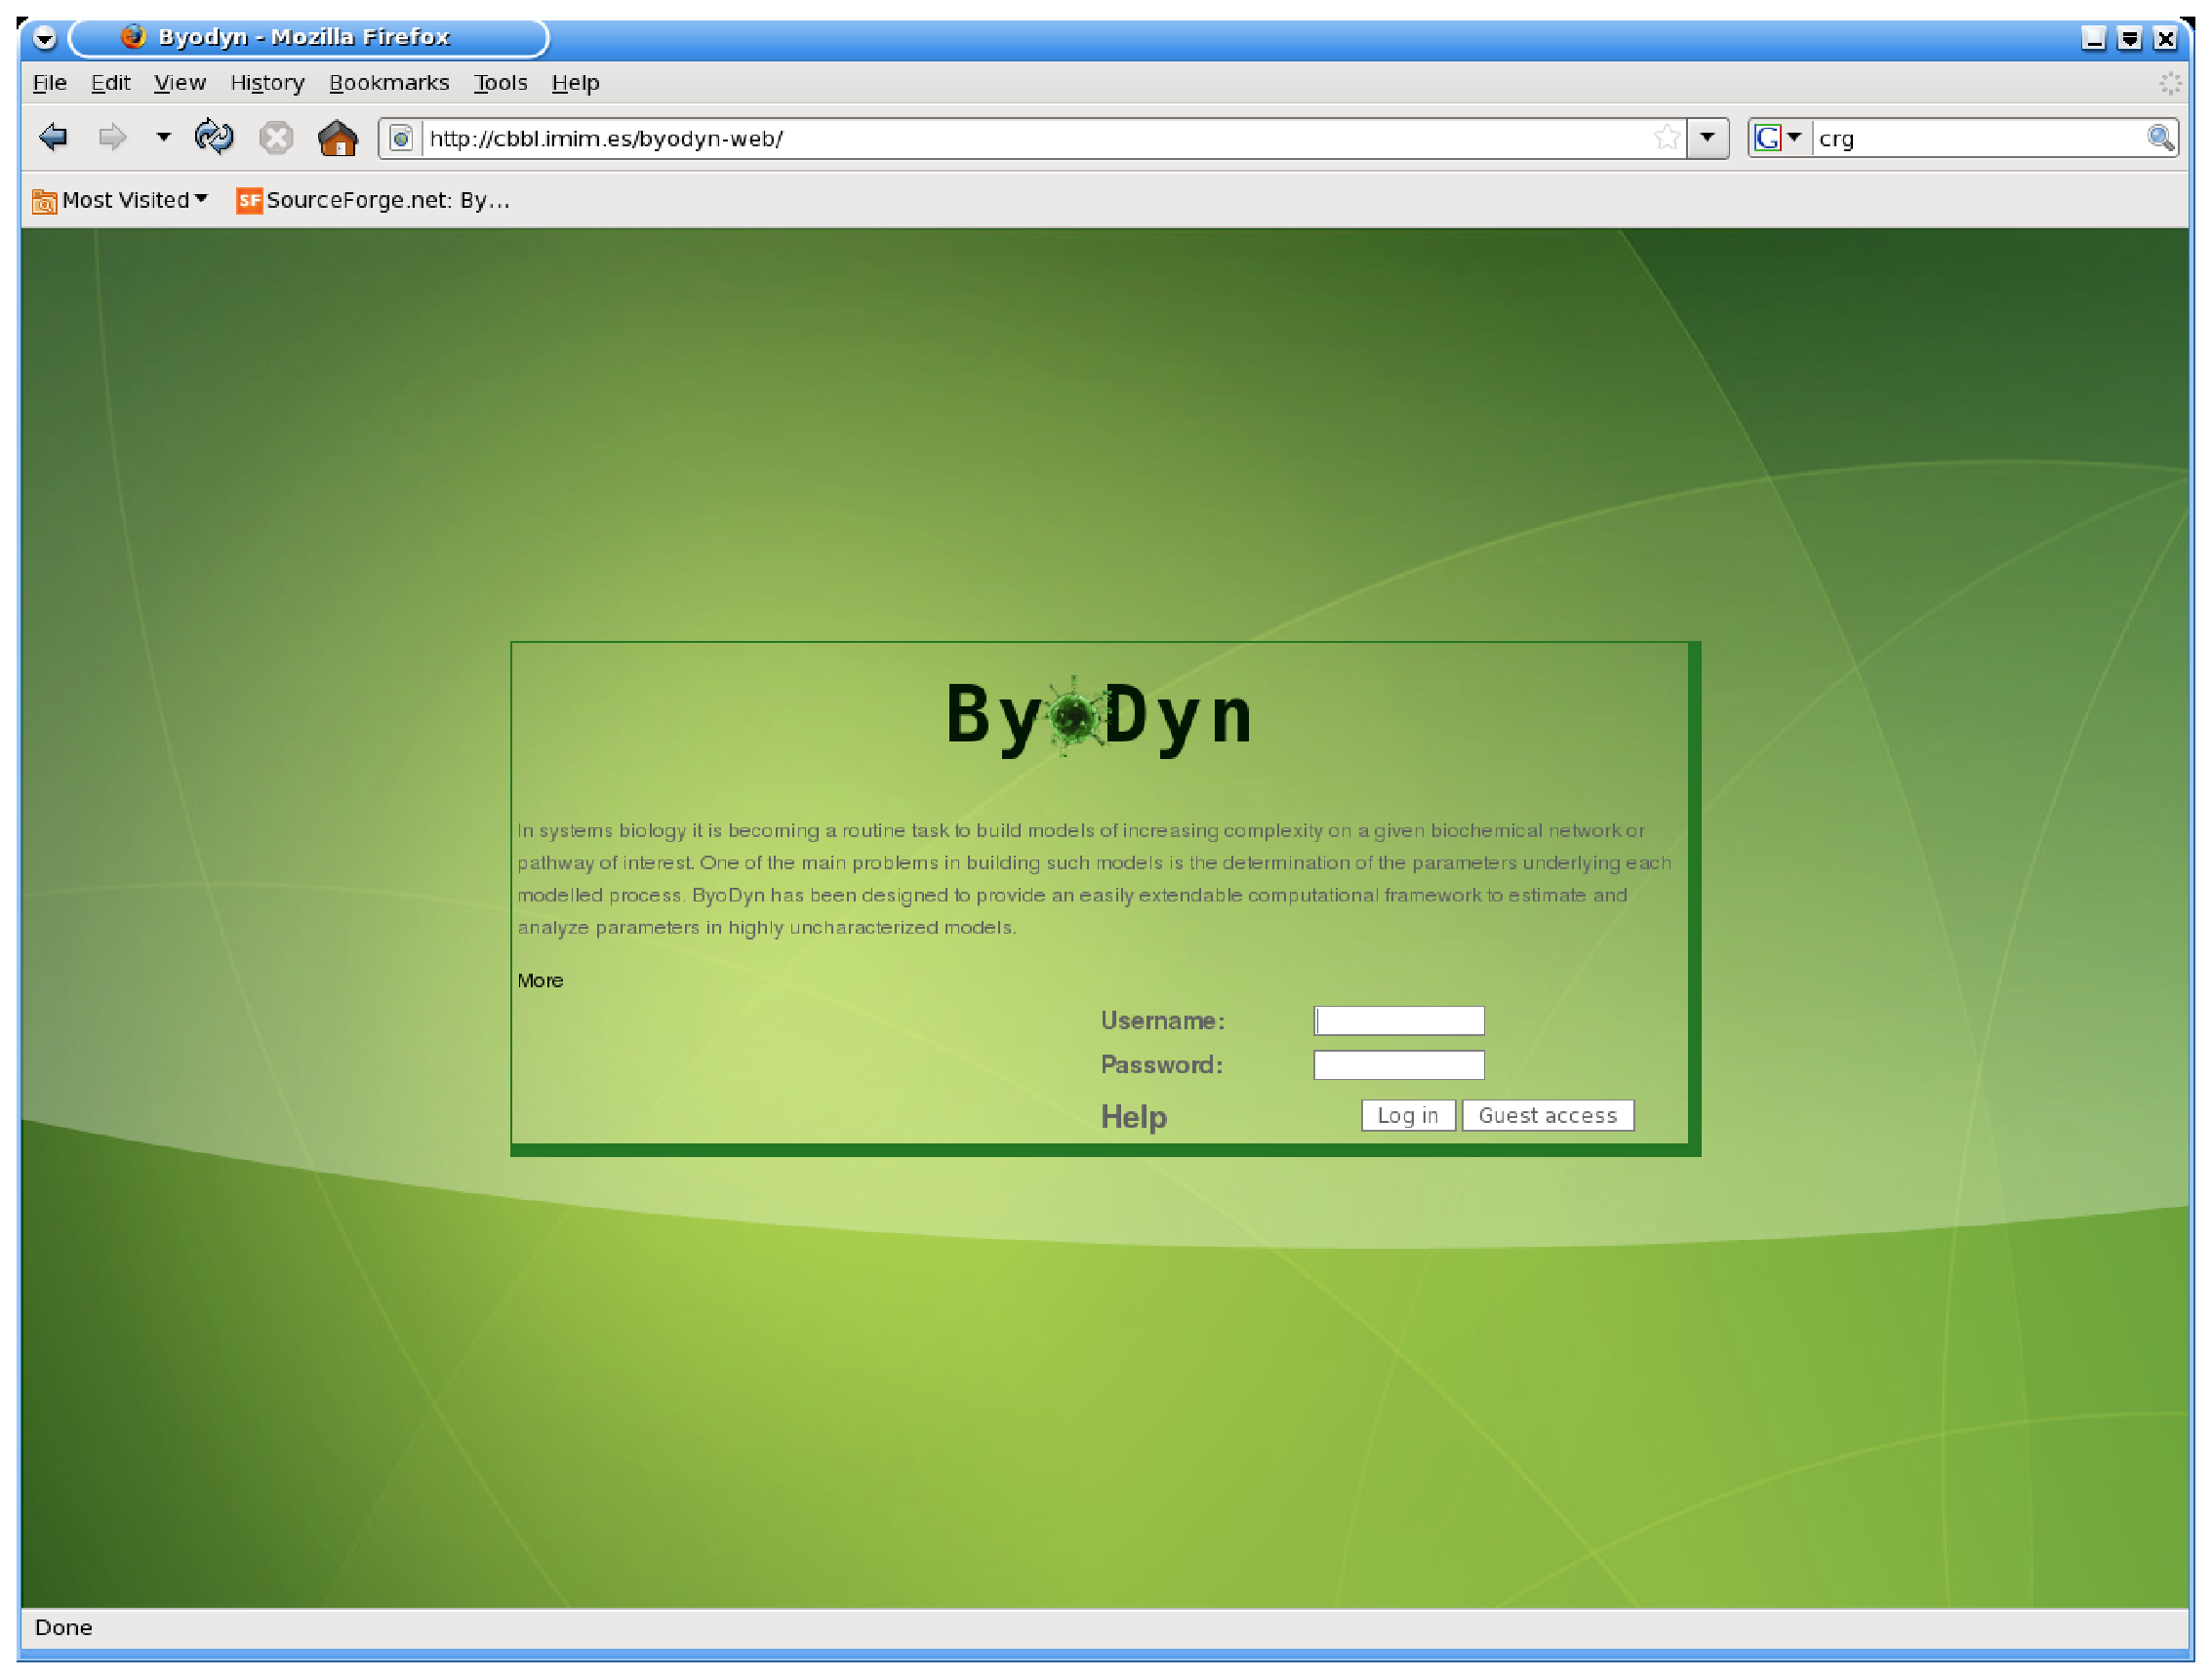
\includegraphics[scale=0.35]{figures/screenShots/frontPage.eps}
      \caption{
        Screenshot of the \texttt{ByoDyn.web} front page.
      }
      \label{frontPage}
    \end{center}
  \end{figure}
  \subsubsection{\texttt{ByoDyn.web} Home}
  The first page that you will see after the front page is called \emph{Home}.
  We also display it, in Figure \ref{home}. 
  The page shows the user workspace, called ``My workspace'', which is a virtual place in the application where your work files (i.e. models, analysis files, results) are stored . 
  The user workspace is divided into three main subsections:
  \begin{itemize}
  \item \textbf{My models:} 
    Here, you can find your models. 
    The models are the computational representations of a biochemical system. 
  \item \textbf{My analysis:} 
    This subsection stores your analysis files. 
    The analysis files are the input files for \texttt{ByoDyn}, which define all the details and instructions in order to run the analysis.
  \item \textbf{My results:} 
    The results of each analysis resulting from the execution of the analysis files will appear and will remain stored in this subsection.
\end{itemize}
  \begin{figure}[ht!]
    \begin{center}
      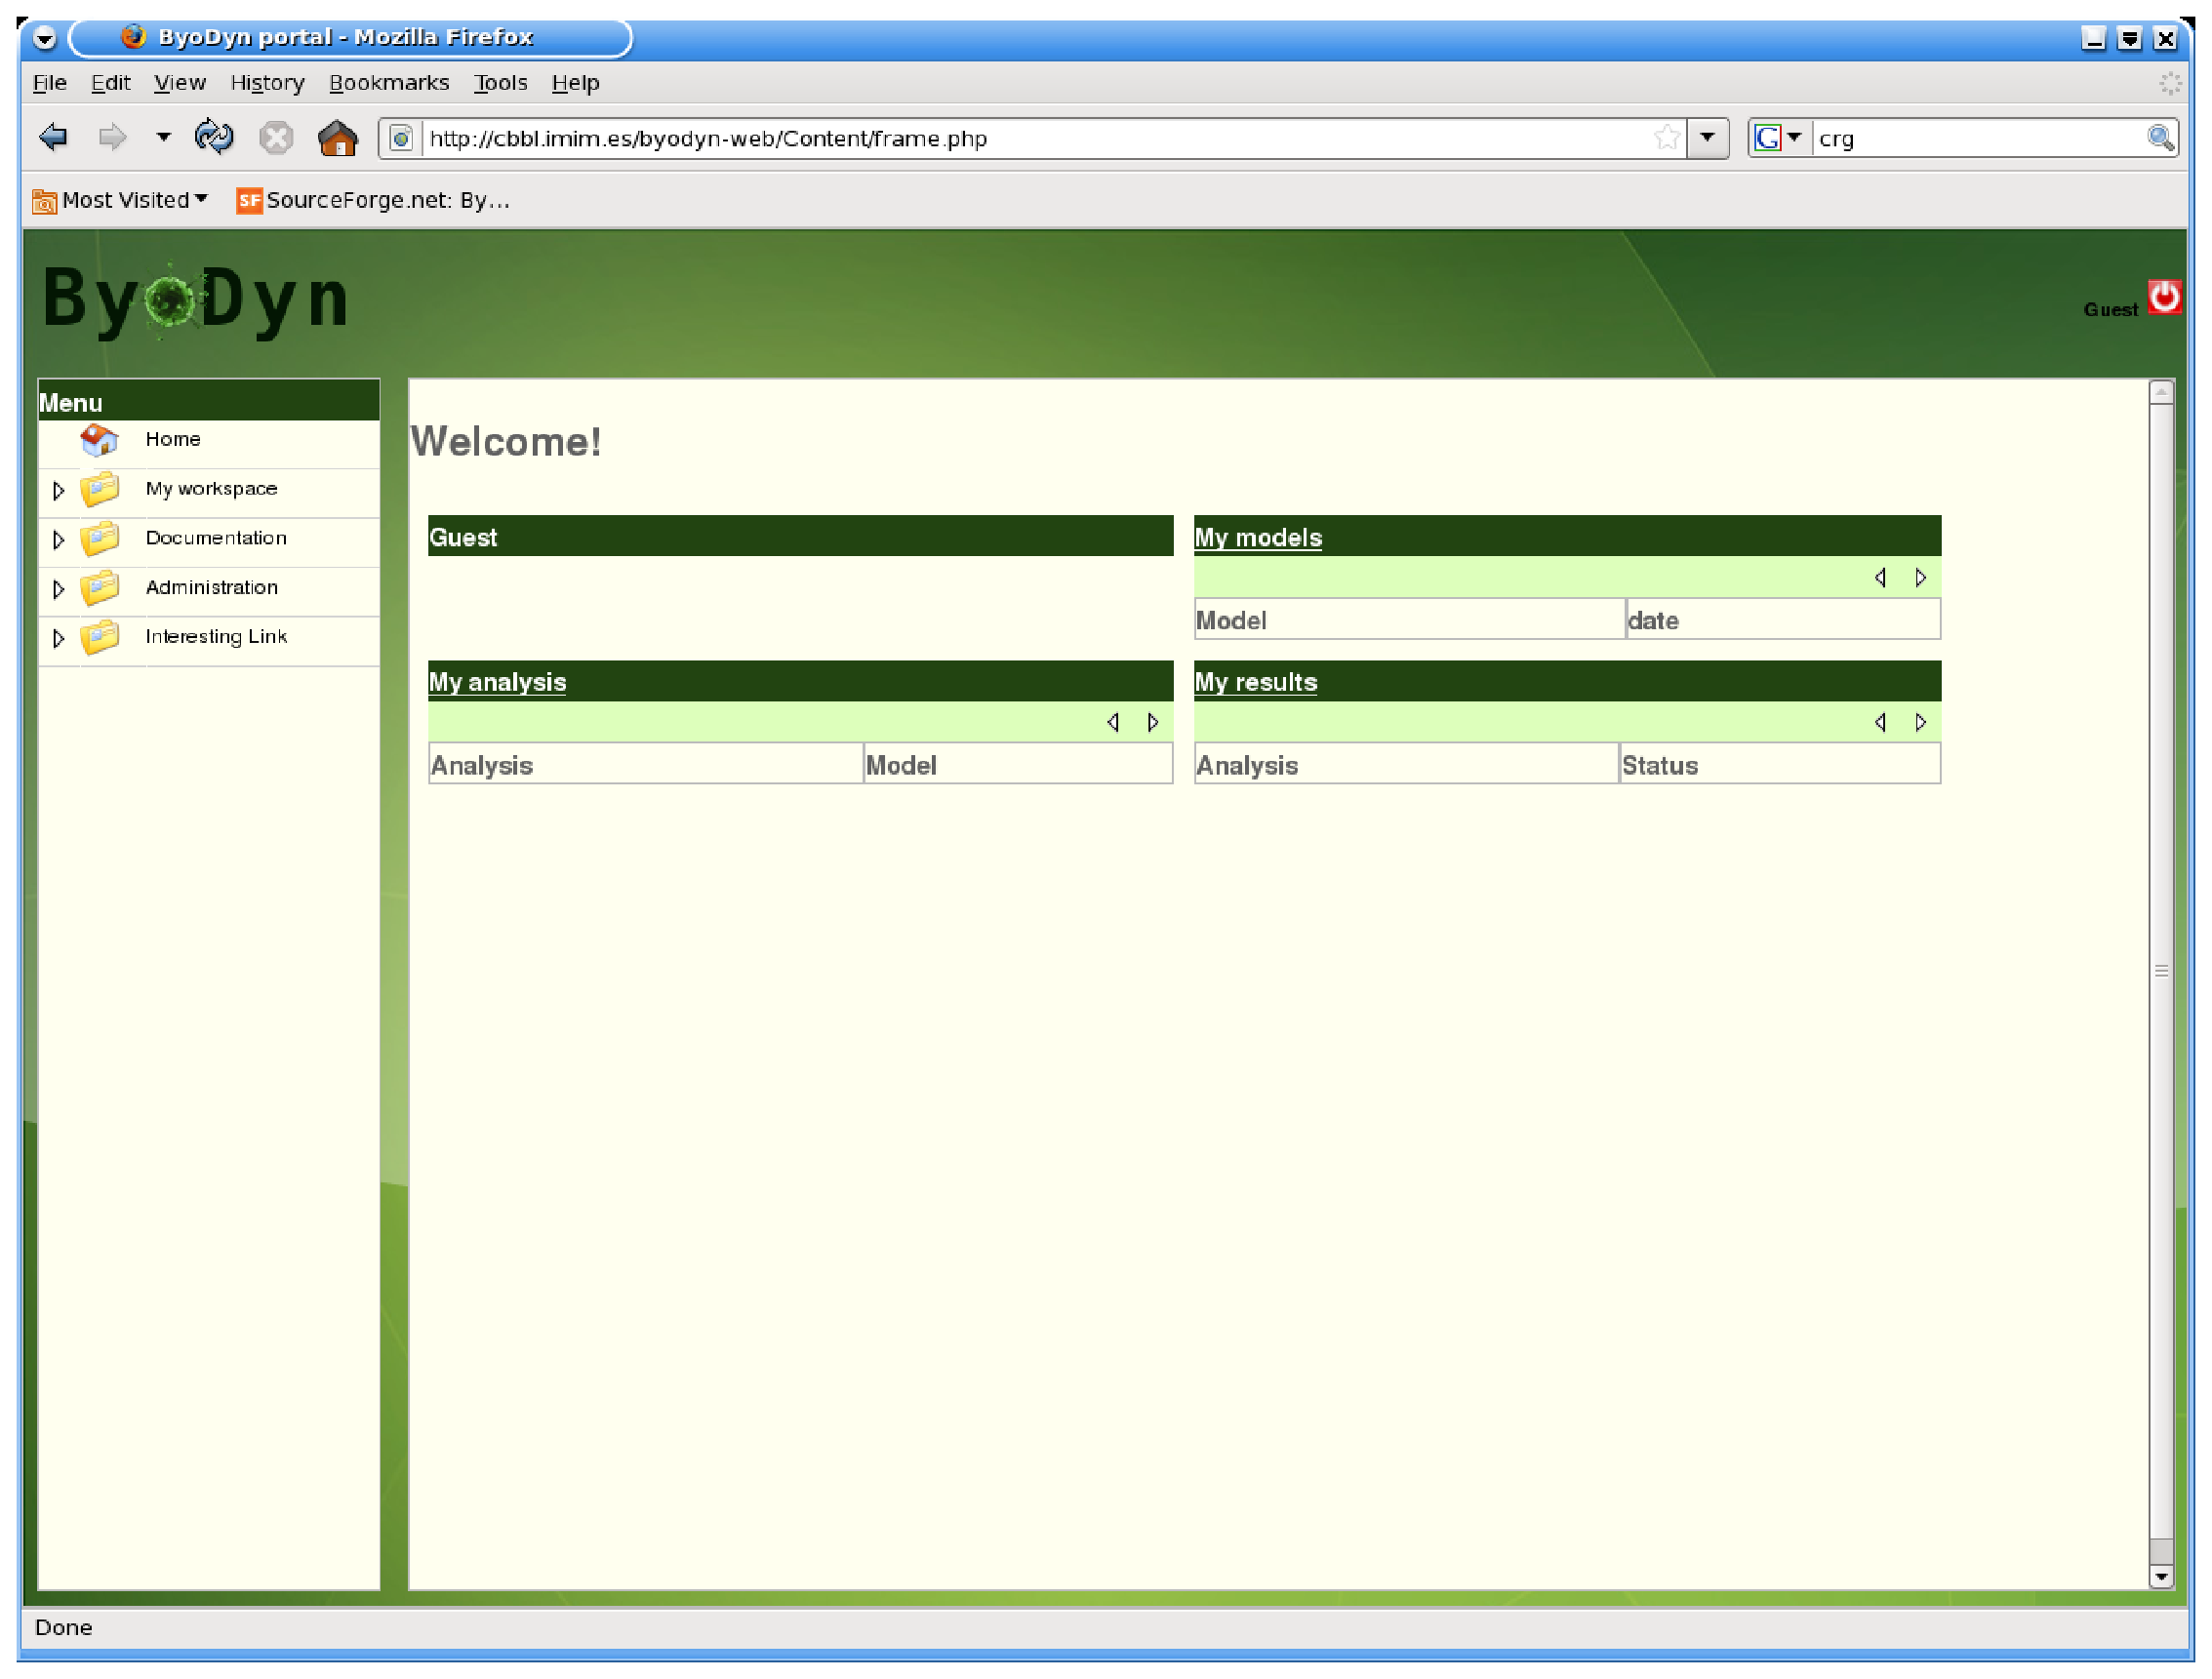
\includegraphics[scale=0.35]{figures/screenShots/home.eps}
      \caption{
        Screenshot of the \texttt{ByoDyn.web} home page.
      }
      \label{home}
    \end{center}
  \end{figure}
  \subsubsection{First Analyses: the Quick Start Examples}
  In Section \ref{functionalities} we explain the different funcionalities \texttt{ByoDyn} offers via a bunch of example files. 
  That section gives detailed explanations about the files and the results of those examples files of your workspace.

  In order to find the example files you should browse along the menu bar at the left side of the screen. 
  There you will find the \textbf{Examples} folder with two subfolders inside:
  \begin{itemize}
  \item \textbf{Option files from documentation:} 
    In this subfolder you can find some analysis files, explained farther in this document, specifically in Section \ref{functionalities}.
  \item \textbf{Models:} 
    Here, you will find biochemical models in SBML format from public repositories.
  \end{itemize}
  Specifically, you need to do the following steps in order to work with the examples shown in Section \ref{functionalities}:
  \begin{itemize}
  \item
    Click on Examples/Option files from documentation/Quick Start of menu bar. 
  \item 
    Now, in the main screen there are a list of files with a green arrow at the left. 
    You need to click on the green arrow in order to copy the specific file on your workspace.
  \item 
    Click on \texttt{Home} in order to return to the home page. 
    Now, you can see in \texttt{My analysis} and in \texttt{My models}, the example files.
  \item 
    Click on the specific analysis file and the details of this file will appear. 
    Here, you could see the analysis file using the \texttt{Visual edition} tab or the \texttt{Text editor} tab.
  \item 
    To execute the analysis please click on the fourth icon from the left, at the top, the one with the \emph{Play} symbol. 
  \item 
    To see the state of the calculation and the results, please click on the last icon at top, the one with the folder symbol.
  \end{itemize}
  This protocol is valid for any of the functionalities explained at the next section.
  \subsection{Common functionalities} \label{functionalities}
  \subsubsection{Exporting}
  Run the command \texttt{byodyn} and the name of the \emph{runner} file, \texttt{exporting.rn} in this case. 
  It will create an \texttt{output} directory with the results. 
  Change to the \texttt{output} directory and you will list a file named \texttt{Kinetic\_modelling\_of\_Amadori\_degradation.xml} containing the new parameter values as defined on the runner file: parameter \texttt{k4v4} takes now 0.07 as value in the new SBML file.
  \subsubsection{Simulation}\label{simulation}
  Run again the command \texttt{byodyn} and the name of the \emph{runner} file, \texttt{simulation.rn}. 
  Change to the \texttt{output} directory and you will list:
  \begin{itemize}
    \item
      \texttt{Kinetic\_modelling\_of\_Amadori\_degradation.description.txt}: A short description of the input model. 
      We state the name of the model, the number of nodes, the number of constant species and the number of constant and non-constant parameters.
    \item
      \texttt{Kinetic\_modelling\_of\_Amadori\_degradation.out}: it is called that way because the given name of the model.
      More important is the extension of the files. 
      This \texttt{.out} is a file with the concentration of each node (in columns) along time (first column).
    \item
      \texttt{Kinetic\_modelling\_of\_Amadori\_degradation.ps}: is equivalent from the former file but represented as a graph.
    \item
      \texttt{Kinetic\_modelling\_of\_Amadori\_degradation.veloc.out}: the same as \texttt{Kinetic\_modelling\_of\_Amadori\_degradation.out} but in this case the columns represent the rate of concentration change for the corresponding node.
    \item
      \texttt{Kinetic\_modelling\_of\_Amadori\_degradation.veloc.ps}: the corresponding graph for the file \\\texttt{Kinetic\_modelling\_of\_Amadori\_degradation.veloc.out}.
    \item
      \texttt{Kinetic\_modelling\_of\_Amadori\_degradation.tex}: it is a file with the system of ODEs and the equations of kinetic laws  in latex format. 
      Just use the program \texttt{pdflatex} to obtain the formulae in pdf format.
    \item
      \texttt{scratch} directory: this is a directory that contains necessary files for \texttt{ByoDyn} but of secondary interest for the user.
      We can list the following files:
      \begin{itemize}
	\item
	  \texttt{Kinetic\_modelling\_of\_Amadori\_degradation.0.integ.py}: this file contains the commands necessary to integrate the system of ODEs using SciPy.
          In the case of using Octave as the program to numerically solve the ODEs, you will find an equivalent \texttt{Kinetic\_modelling\_of\_Amadori\_degradation.0.oc}.
          The number refers to the rank of the processor in parallel machines.
	\item
	  \texttt{Kinetic\_modelling\_of\_Amadori\_degradation.gnu}: the \texttt{gnuplot} commands necessary to build the \texttt{.ps} files from the \texttt{.out}.
	\item
	  \texttt{Kinetic\_modelling\_of\_Amadori\_degradation.veloc.gnu}: the same but for the velocities instead of the concentrations.
      \end{itemize}
  \end{itemize}
  If you have a look to the to the \emph{runner} file (Fig. \ref{simulationRunner}), here is an explanation about the different option fields:
  \begin{figure}[ht!]
    \begin{center}
      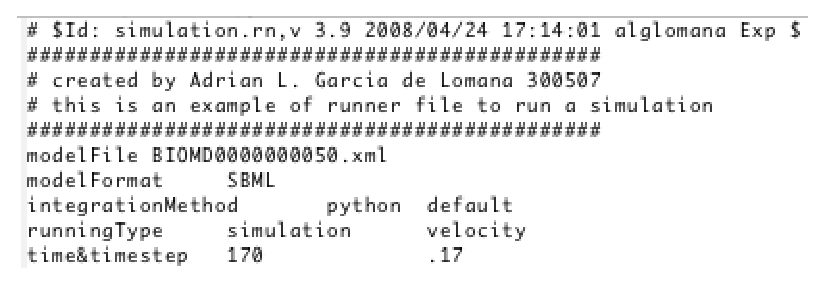
\includegraphics[scale=.75]{figures/simulationRunner.eps}
      \caption{
        Snapshot of a \emph{runner} file example for a deterministic simulation.
      }
      \label{simulationRunner}
    \end{center}
  \end{figure}
  \begin{itemize}
    \item
      \texttt{modelFile}: you need to specify the name of the \emph{model} file.
      If the file is not at the same directory that the one from where you are running \texttt{ByoDyn}, set the complete path, for example:\\
      \texttt{/home/myself/myfolder/examplesOfByoDyn/myinput.xml}
    \item
      \texttt{modelFormat}: this defines the format of the \emph{model} file.
      There are two possibilities, either \texttt{SBML} or \texttt{tags}.
    \item
      \texttt{integrationMethod}: this variable sets the program you want to use to solve the system of ordinary differential equations (ODEs) created by \texttt{ByoDyn}. There are two main possibilities that are specified at the first field: either \texttt{python} to use SciPy or \texttt{octave} to use Octave. The second field refers to the integration method being as possibilities \texttt{default}, \texttt{adams}, \texttt{non-stiff}, \texttt{bdf} or \texttt{stiff}. See the Reference Manual for further theoretical information about what these methods do. However, if you do not have any preference, you can adjust the first field with the option \texttt{automatic} instead of \texttt{python} or \texttt{octave}.
    \item
      \texttt{runningType}: the different possibilities are \texttt{runningType} are \texttt{exporting}, \texttt{simulation}, \texttt{parameterEstimation}, \texttt{calculateFunction}, \texttt{dynamicsReconstruction}, \texttt{scoreSurface}, \texttt{sensitivityAnalysis}, \texttt{identifiabilityAnalysis} or \texttt{optimalExperimentalDesign}.  
      In the case of a simulation, another field has to be append: either \texttt{velocity} or \texttt{noVelocity} to choose if you also require information of the velocity of the concentration change of the nodes along time.
    \item
      \texttt{time\&timestep}: clearly you have to set the simulation time and the time step used by the simulation.
  \end{itemize}
  \subsubsection{Stochastic Simulation} \label{stochastic}
  If you want to run a stochastic simulation execute \texttt{ByoDyn} with the option file \texttt{stochastic.rn}.
  The option file is shown in Figure \ref{stochasticRunner} and we highlight here the differences from a deterministic simulation:
  \begin{figure}[th!]
    \begin{center}
      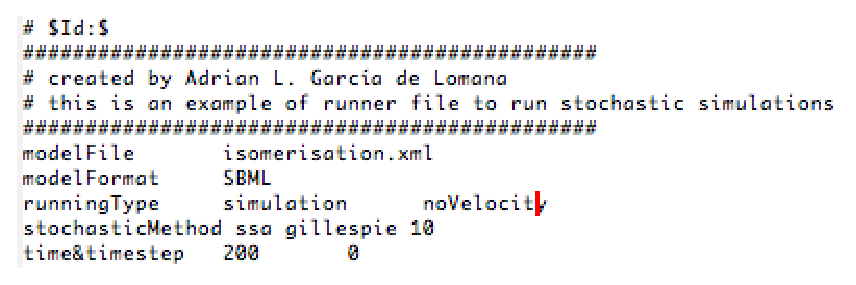
\includegraphics[scale=.75]{figures/stochasticRunner.eps}
      \caption{
        Snapshot of a \emph{runner} file example for a stochastic simulation.
      }
      \label{stochasticRunner}
    \end{center}
  \end{figure}
  \begin{itemize}
    \item 
      \texttt{stochasticMethod}: this variable replaces \texttt{integrationMethod} and should be specified in order to run a stochastic simulation.
      Two algorithms are available, Gillespie and $\tau$-leap.
      The respective arguments are \texttt{ssa gillespie} and \texttt{tau-leap default}. 
      A further more argument is required in both cases, an integer, defining the number of runs that should be launched.
    \item
     \texttt{time\&timestep}: for the case of the $\tau$-leap algorithm the meaning of \texttt{time\&timestep} is the same as for the deterministic simulations, but please consult the user reference manual for the interpretation of \texttt{time\&timestep} in the case of the Gillespie algorithm.
  \end{itemize}
  The output of the stochastic simulations is very similar to the one of the deterministic simulations, however, there are some minor differences which are described again at the user reference manual.
  \subsubsection{Optimisation}  \label{optimisationSection}
  One of the most appealing functionalities of \texttt{ByoDyn} is the model parameter identification from time course experimental data using optimisation techniques. The User Reference Manual is pointed for more details about the algorithms used, the minimizing function and other issues of theoretical interest.
  In this case we present an optimisation of the 5 most sensitive parameters.
  One order of magnitude up and down for each parameter is specified as possible range for parameter exploration.
  Hybrid optimisations are composed of a global optimisation and a local optimisation algorithm.
  The local optimisation routines are written in Fortran and have to be compiled first.
  \paragraph{Two Phases Hybrid Optimisation}
  In the case of a two phases hybrid algorithm, the global optimisation runs until a certain condition is accomplished.
  At this point, it is assumed that the parameter vector is at the region of the global minimum and a local search is initialized for a quick convergence.
  In order to launch the optimisation, we have to use the file \texttt{optimisation.rn}.
  The optimisation lasts for several minutes depending on the machine and the optimisation evolution. 
  It is a stochastic algorithm and the computational cost may vary largely. 
  In our tests on a 1.83 GHz Intel Core Duo the optimisation took around two minutes of CPU time.

  We understand a successful calibration of the parameters when the values retrieved from the optimisation match with the ones used to generate the trajectories. 
  In a realistic situation, where the nominal value of the parameters is not known \textit{a priori}, the final value of the fitness function can be useful to rank the obtained solutions and discriminate the most plausible values as there are several orders of magnitude of difference between a local minimum and a global minimum. 
  In our case local minima were in the range of 10$^4$ while the global minimum is at a value of 10$^{-16}$.
  Obviously the fitness function value for an experimental calibration is not known, but huge differences should be observed when ranking the solutions.

  Let's have a look to the resulting new files at the \texttt{output} directory:
  \begin{itemize}
    \item
      \texttt{Kinetic\_modelling\_of\_Amadori\_degradation.st}: this file contains for each generation of the GA algorithm the mean value of the population and the value of the best individual.
    \item 
      \texttt{Kinetic\_modelling\_of\_Amadori\_degradation} directory: when a solution has been found, a directory named as the input model is created. 
      Two directories containing equivalent files will be found: \texttt{parametersFromGA} and \texttt{parameterFromHybridTwoPhases} directories.
      At these directories you an find several files named as the parameter you set to identify. 
      The structure is the following: the first column is the value of the parameter, the other two the range in which the parameter space has been explored and the last one the value of the fitness function. 
      Keep in mind that the starting points of the local search are the final values of the GA.
      It is worth to note that the fitness function of the results from the local search are orders of magnitude  better than the ones of the GA.
      Also the resulting values of the parameters are very close to the nominal values (the values for which the fitting data was generated), in this case: $k10$ = 0.0707, $k16$ = 0.0134, $k3$ = 0.0155, $k2$ = 0.0156 and $k1$ = 0.0057.
      \item
	\texttt{scratch} directory: apart from the known \\ \texttt{Kinetic\_modelling\_of\_Amadori\_degradation.0.integ.py} there is a directory called \texttt{localSearch\textit{x}} being \textit{x} a number of 12 digits. 
	This directory contains several files for the local search.  
	More information is given at the Reference Manual.
  \end{itemize}
  The runner file used is shown in Fig. \ref{singleOptimisationRunner}.
  \begin{figure}[t]
    \begin{center}
      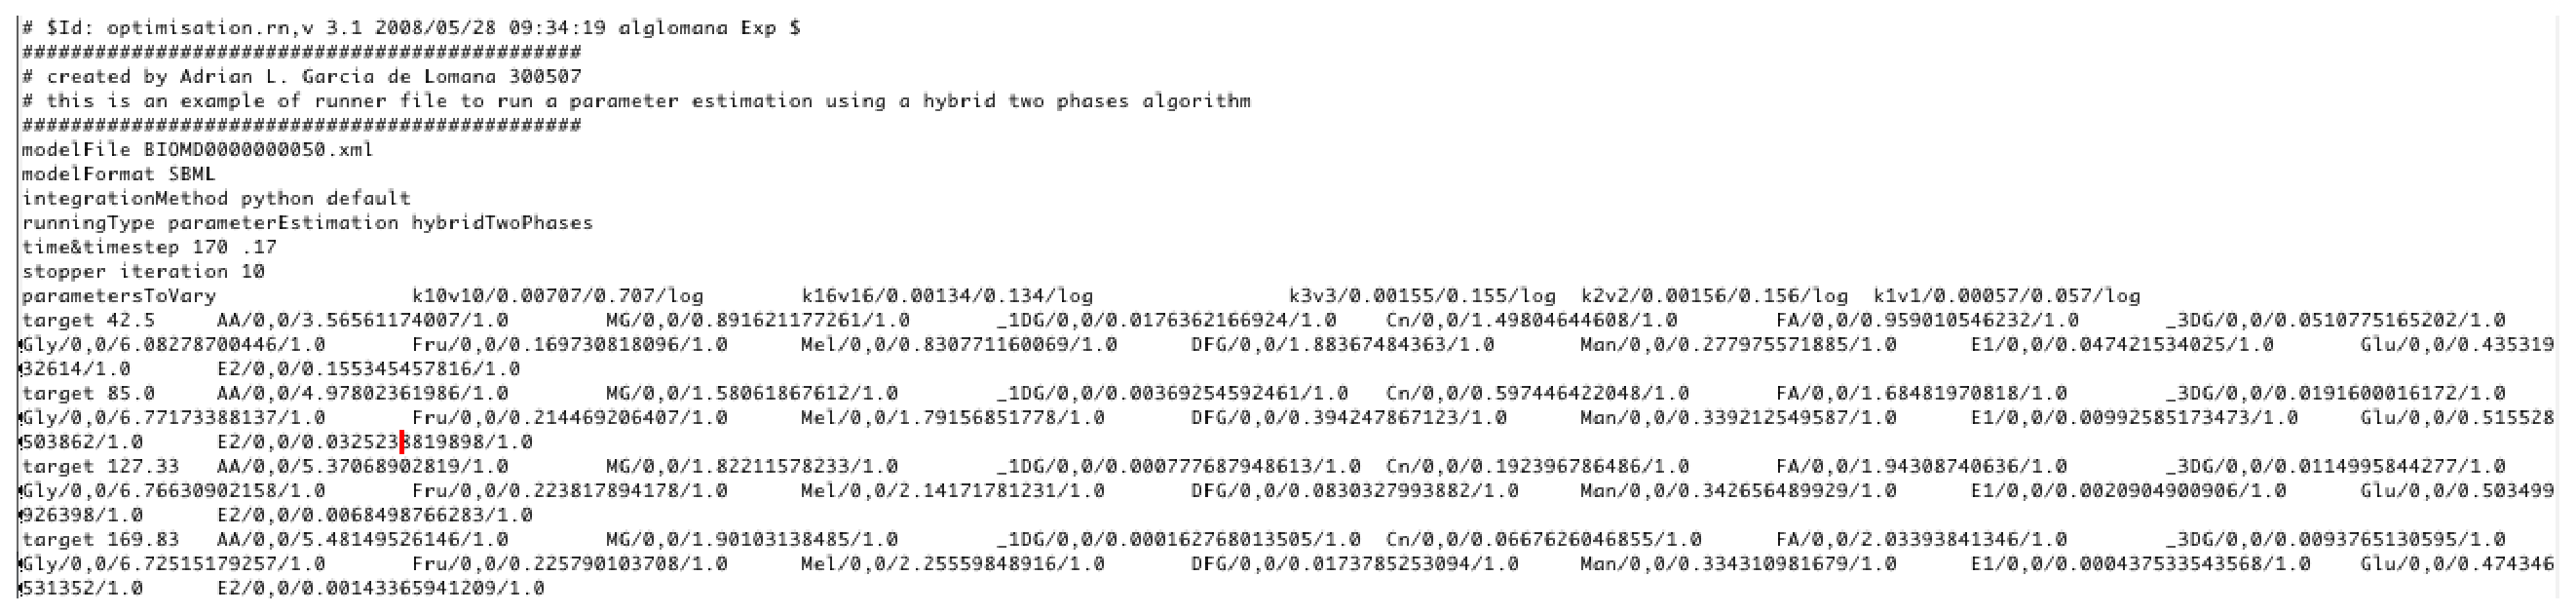
\includegraphics[scale=.38]{figures/optimisationRunner.eps}
      \caption{Snapshot of the \emph{runner} file example to perform a parameter estimation.}
      \label{singleOptimisationRunner}
    \end{center}
  \end{figure}
  Compared to the \emph{runner} file of the simulation (Figure \ref{simulationRunner}), the new fields are the following:
  \begin{itemize}
  \item
    \texttt{stopper}: this variable controls when to stop the optimisation. 
    In this case we set a number of generations for the GA.
    But it is possible also to set a value of the fitness function as threshold to have more control over the parameter space we are searching. 
    More information is given at the Reference Manual.
  \item
    \texttt{parametersToVary}: Very similar to the field of \texttt{sensitivityParameters} from the sensitivity analysis, with two exceptions.
    \begin{itemize}
      \item
	\textit{A boundary has to be set}: the algorithm will explore the parameter space at that range of values.
	The first value has to be smaller that the upper value.
      \item
	\textit{Search scale}: When the searching range is wide (orders of magnitude) it has to be explored in a logarithmic scale so the distribution is not biased to the large values.
	If the parameter to be identify is an exponent, where the typical range of values is from $1.0$ to $10.0$, the linear scale is preferred.
	This is expressed by the tag \texttt{log} or \texttt{lin} respectively.
    \end{itemize}
    All of it separated by a $/$ as shown in the Figure \ref{singleOptimisationRunner}.
  \item
    \texttt{target}: this field refers to the (experimental) temporal expression data that we want to fit.
    The structure is the following: for a given time, you define the expression value by selecting a node, a cell, the concentration value and the standard deviation of the measurement. 
    In our case the \emph{experimental} data is produced \textit{in silico} then each value comes from a single \emph{measurement} and the value of the standard deviation is set as $1.0$.
    The system is composed of a single cell so the cell index in the tissue matrix is the $0,0$.
    As you can observe, several nodes can be fitted at a given time, but this is not a requirement.
  \end{itemize}
  \subsubsection{Fitness Function Calculation}
  If the field \texttt{target} is defined as in Section \ref{optimisationSection}, you can quickly know the distance from you model calling this functionality.
  The runner file you need is shown in Fig. \ref{ffcRunner}.
  \begin{figure}[t]
    \begin{center}
      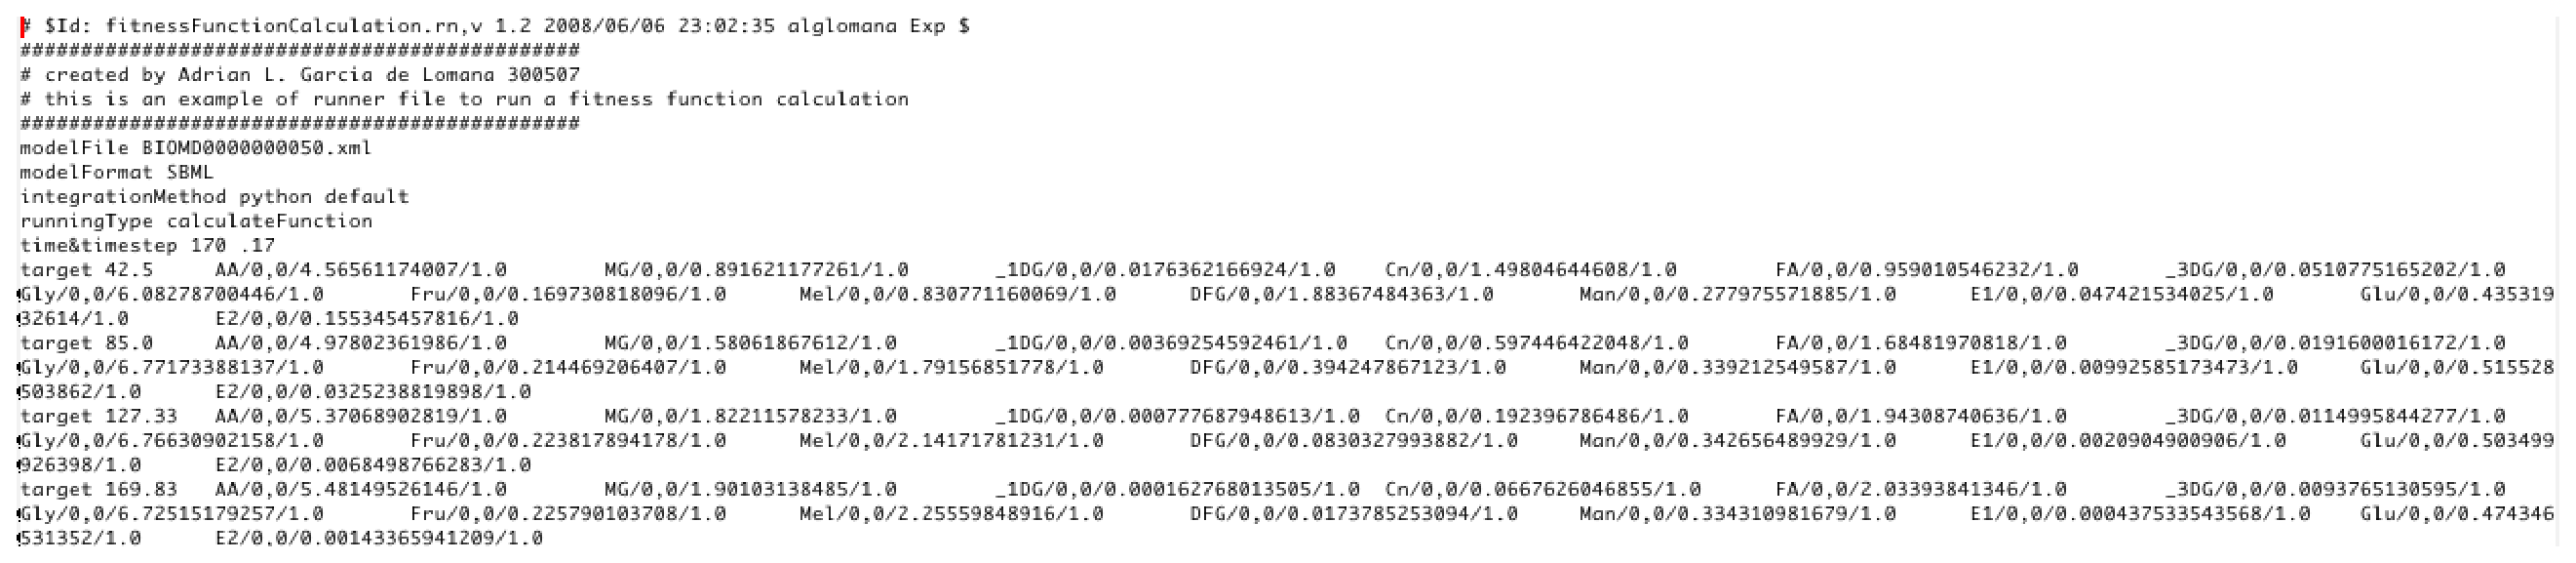
\includegraphics[scale=.38]{figures/ffcRunner.eps}
      \caption{Snapshot of the \emph{runner} file example to perform a fitness function calculation.}
      \label{ffcRunner}
    \end{center}
  \end{figure}
  \subsubsection{Trajectories Reconstruction}
  After launching a parameter estimation, you end up with a bunch of solutions.
  In order to get an idea of how behave the new models you can define a directory where the files of the parameter solutions are stored and \texttt{ByoDyn} will reconstruct the trajectories corresponding to the parameter values.
  See Fig. \ref{trRunner} for a snapshot of the runner.
  The constrains defined on the \texttt{target} are also plotted.
  Furthermore, an interesting detail is that the trajectories reconstructed using the first value of the files is highlighted on the graph depicted as a dark thik line. 
  We suggest to add as first line the original value of the model parameters to have an idea of the change of the model behaviour after the model calibration.
  \begin{figure}[t]
    \begin{center}
      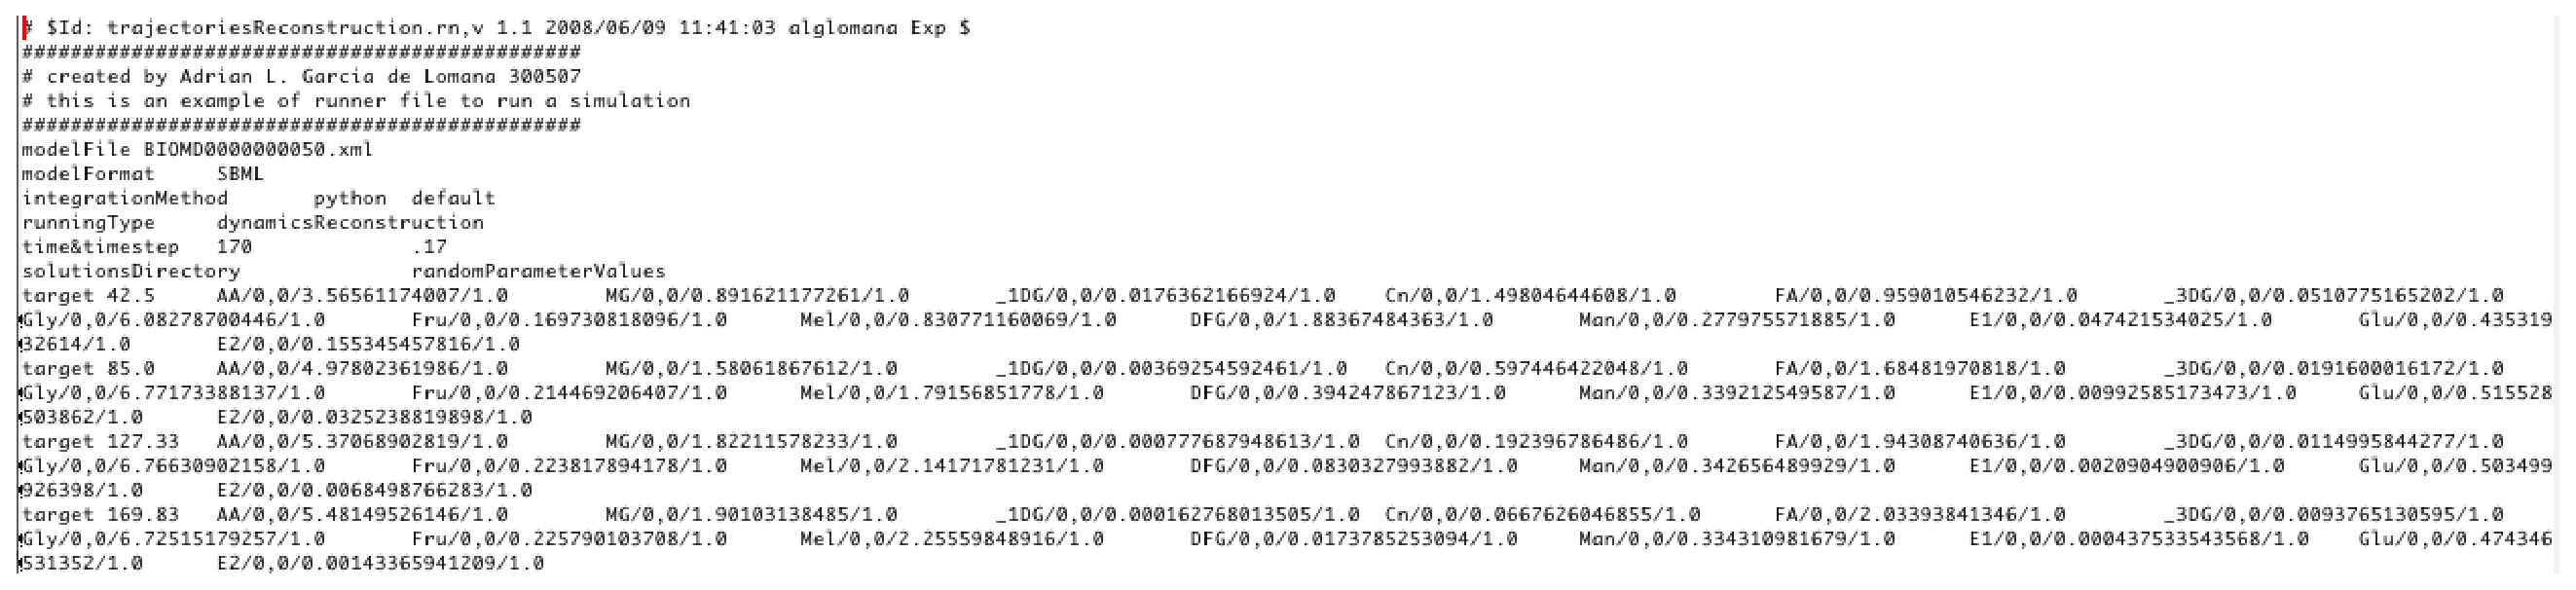
\includegraphics[scale=.38]{figures/trRunner.eps}
      \caption{Snapshot of the \emph{runner} file example to perform the trajectories reconstruction.}
      \label{trRunner}
    \end{center}
  \end{figure}
  \subsubsection{Fitness Function Surfaces}
  If we are interested to know the fitness function values in the surroundings of a given parameter point, the result of an optimisation for example, we can build a surface in the parameter space.
  In the \texttt{output} directory we have two new files not described previously:
  \begin{itemize}
    \item \texttt{k1.k2.txt}: this text file contains a matrix for the values of the fitness function surface.
    \item \texttt{k1.k2.ps}: this file is a postscript plot with the surface.
      The color indicates the fitness function value.
      The range of the parameters is shown.
  \end{itemize}
  The runner file looks as shown in Figure \ref{surfaceRunner}.
  \begin{figure}[t]
    \begin{center}
      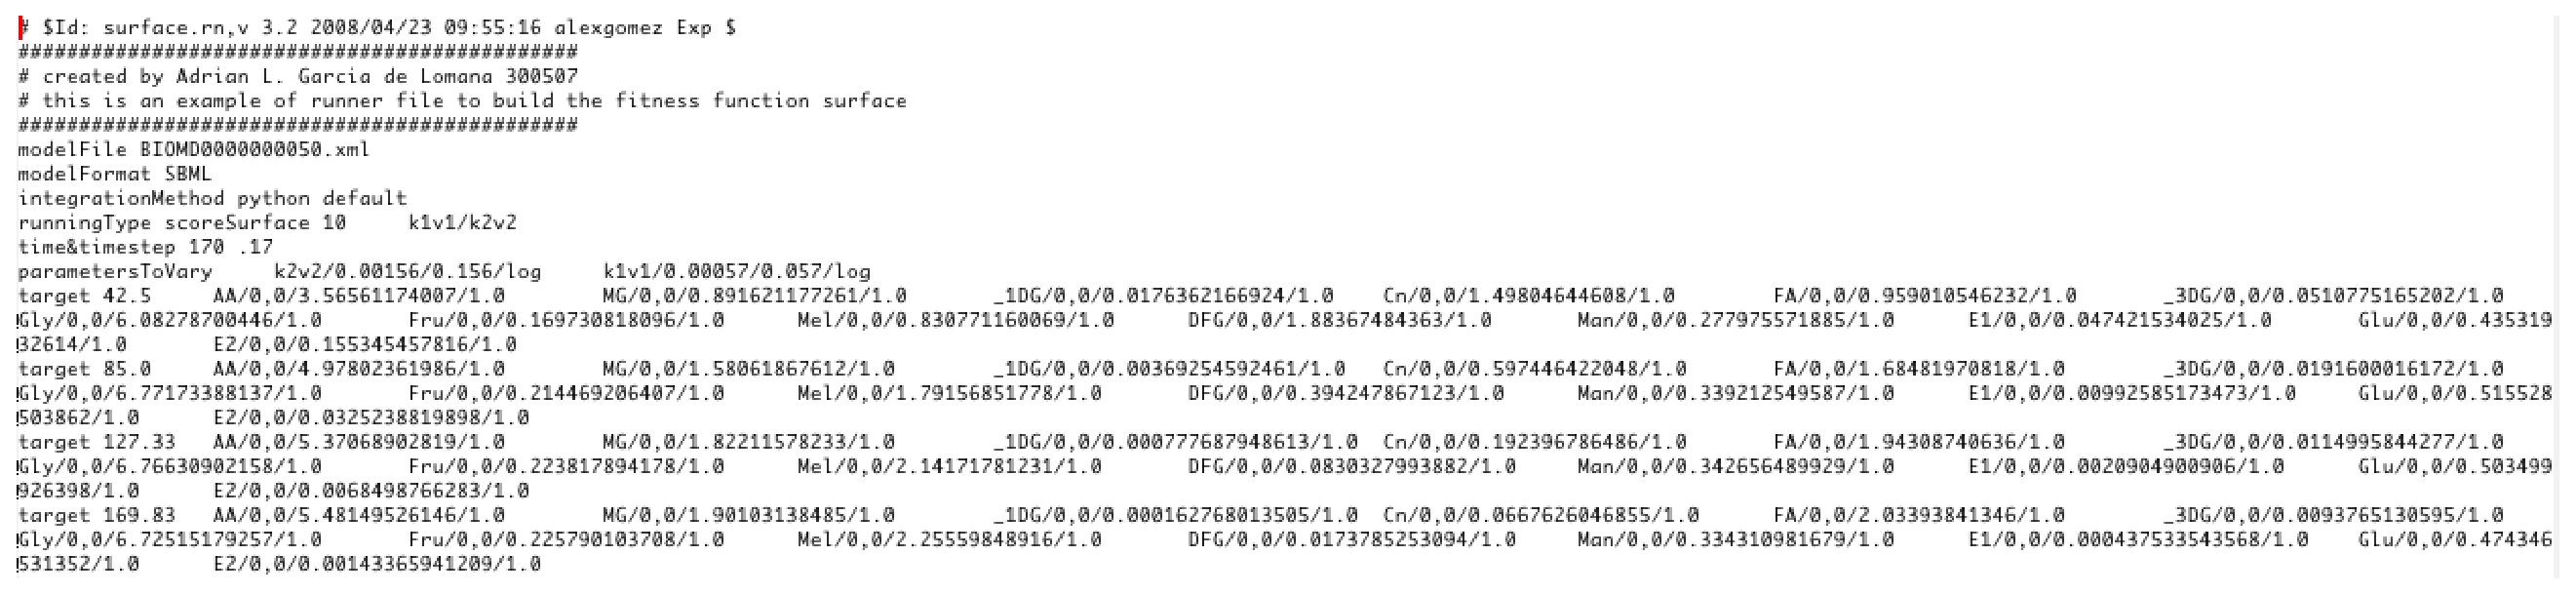
\includegraphics[scale=.38]{figures/surfaceRunner.eps}
      \caption{Snapshot of the \emph{runner} file example to perform a fitness function surface.}
      \label{surfaceRunner}
    \end{center}
  \end{figure}
  \subsubsection{Sensitivity Analysis}
  In order to perform a sensitivity analysis you have to run \texttt{ByoDyn} using the \emph{runner} file called \texttt{sensitivity.rn}.
  Again the results are in the folder called \texttt{output} and you could examine the following files:
  \begin{itemize}
  \item
    \texttt{Kinetic\_modelling\_of\_Amadori\_degradation.ps} and \\ \texttt{Kinetic\_modelling\_of\_Amadori\_degradation.out} with the same meaning as the one explained in Section \ref{simulation}.
  \item
    \texttt{Kinetic\_modelling\_of\_Amadori\_degradation.sens.global.timeCourse.ps}: this graph represents the sensitivity of the system along time with respect to each of the model parameters. Check the Reference Manual for further information and the formula used.
  \item
    \texttt{Kinetic\_modelling\_of\_Amadori\_degradation.sens.global.txt}: this is a text file containing the global sensitivity of the parameters in order.
  \item
    \texttt{Kinetic\_modelling\_of\_Amadori\_degradation.sens.relative.ps}: this postscript file shows a matrix of the node relative sensitivity of each parameter.
    The intensity of the color is normalised against the maximum value for the model.
  \item
    \texttt{Kinetic\_modelling\_of\_Amadori\_degradation.sens.relative.txt}: this text file holds the same information that the one shown in \\ \texttt{Kinetic\_modelling\_of\_Amadori\_degradation.relative.sens.ps}.
  \item
    \texttt{scratch} directory: as at the simulation, the files called \\ \texttt{Kinetic\_modelling\_of\_Amadori\_degradation.gnu} \\ and \texttt{Kinetic\_modelling\_of\_Amadori\_degradation.0.integ.py} exist with the same meaning as before. 
    Other files specific from the sensitivity analysis are:
    \begin{itemize}
    \item
      \texttt{Kinetic\_modelling\_of\_Amadori\_degradation.\textit{parameter}.out} where \textit{parameter} is the name of the corresponding parameter of the system. 
      These files store the values of the simulations in which the value of the corresponding parameter has been incremented infinitesimally. 	    
    \item
      \texttt{Kinetic\_modelling\_of\_Amadori\_degradation.sens.global.out}: this is the data for the corresponding graph \\ \texttt{Kinetic\_modelling\_of\_Amadori\_degradation.global.sens.timeCourse.ps} at the \texttt{output} directory.
    \item
      \texttt{Kinetic\_modelling\_of\_Amadori\_degradation.sens.global.gnu}: the commands for the plot \\ \texttt{Kinetic\_modelling\_of\_Amadori\_degradation.global.sens.timeCourse.ps} using the data from \texttt{Kinetic\_modelling\_of\_Amadori\_degradation.sens.global.out}.
    \end{itemize}
  \end{itemize}
  The \emph{runner} file we have used (Fig. \ref{sensitivityRunner}) is slightly different from the one of the simulation:
  \begin{figure}[t]
    \begin{center}
      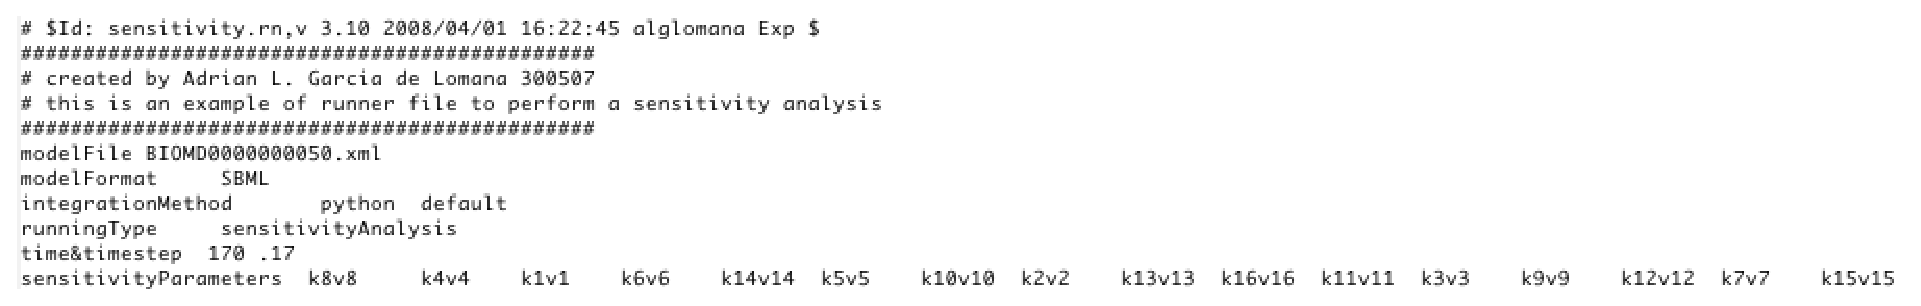
\includegraphics[scale=.75]{figures/sensitivityRunner.eps}
      \caption{
        Snapshot of a \emph{runner} file example for running a sensitivity analysis.
        Note that for format reasons, not all parameters are shown but the sensitivity analysis includes all the parameters of the model.
      }
      \label{sensitivityRunner}
    \end{center}
  \end{figure}
  \begin{itemize}
  \item
    The field of \texttt{runningType}, where you specify that you want to perform a sensitivity analysis by setting the variable to \texttt{sensitivityAnalysis}.
  \item
    \texttt{sensitivityParameters}: You have to define for which parameters you want to study the sensitivity of the system.
  \end{itemize}  
  Finally, other additional files are created in the \texttt{scratch} directory.
  \subsubsection{Identifiability Analysis}
  It is also possible to run an identifiability analysis with \texttt{ByoDyn}.
  Apart from the \texttt{Kinetic\_modelling\_of\_Amadori\_degradation.out} and \\ \texttt{Kinetic\_modelling\_of\_Amadori\_degradation.ps} files described in Section \ref{simulation}, we have the following files specific of the identifiability analysis:
  \begin{itemize}
  \item \texttt{Kinetic\_modelling\_of\_Amadori\_degradation.criteria.txt}: A text file with the final value of the identifiability for the different criteria.
  \item \texttt{Kinetic\_modelling\_of\_Amadori\_degradation.FIM.txt}: A text file containing the Fisher information matrix. Please refer to the User Reference Manual for further information.
  \item \texttt{Kinetic\_modelling\_of\_Amadori\_degradation.COV.txt}: A text file with the inverse of the Fisher information matrix.
  \item \texttt{Kinetic\_modelling\_of\_Amadori\_degradation.correlation.txt}: The correlation matrix of the parameters in text format.
  \item \texttt{Kinetic\_modelling\_of\_Amadori\_degradation.correlation.ps}: This plot shows the correlation of the parameters.
    Blue colours show anticorrelation and red colour positive correlation.
    The intensity of the color is relative to the diagonal of the matrix.
  \end{itemize}
  The input file to run an identifiability analysis is shown in Figure \ref{identifiabilityRunner}.
  Note that in the \texttt{scratch} directory, several files named \\ \texttt{Kinetic\_modelling\_of\_Amadori\_degradation.xx.out}, where xx is the name of one of the parameters of the model, are created necessary to calculate the sensitivity of the model with respect to that parameter.
  \begin{figure}[t]
    \begin{center}
      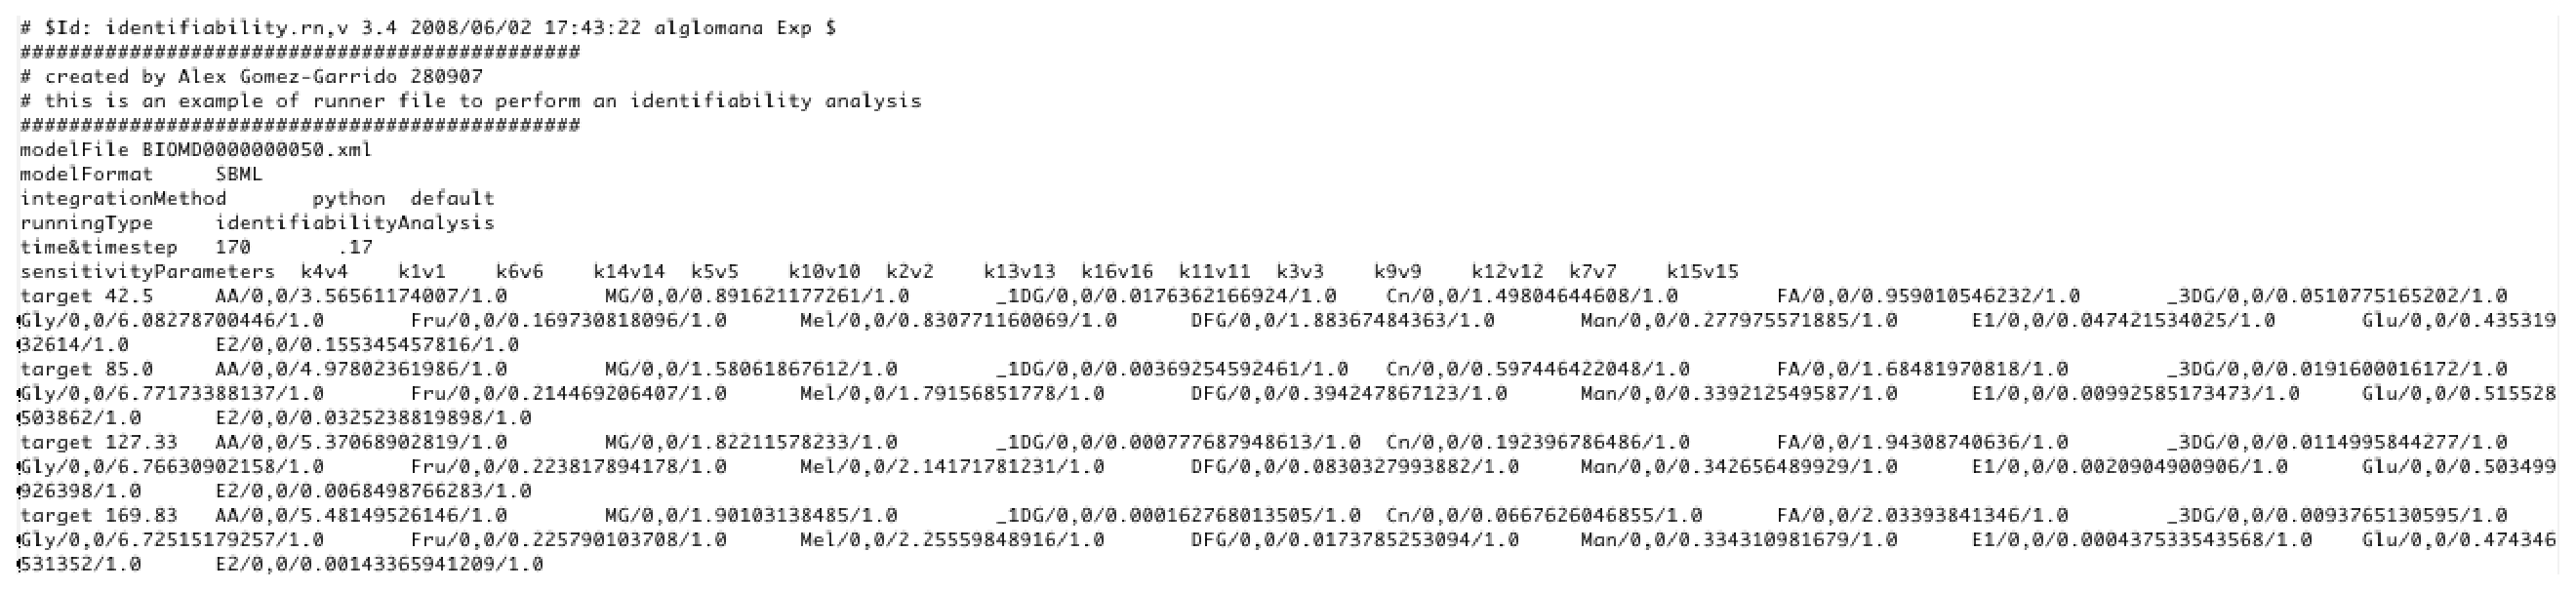
\includegraphics[scale=.75]{figures/identifiabilityRunner.eps}
      \caption{
        Snapshot of an example of \emph{runner} file for running an identifiability analysis.
        Note that for format reasons, not all parameters are shown but the identifiability analysis includes all the parameters of the model.
      }
      \label{identifiabilityRunner}
    \end{center}
  \end{figure}
  \subsubsection{Optimal Experimental Design}
  Optimal experimental design (OED) tells you which would be the next temporal constrain so the identifiability problem becomes more tractable.
  Use a runner file similar to the one shown in Fig. \ref{oedRunner}.
  \begin{figure}[t]
    \begin{center}
      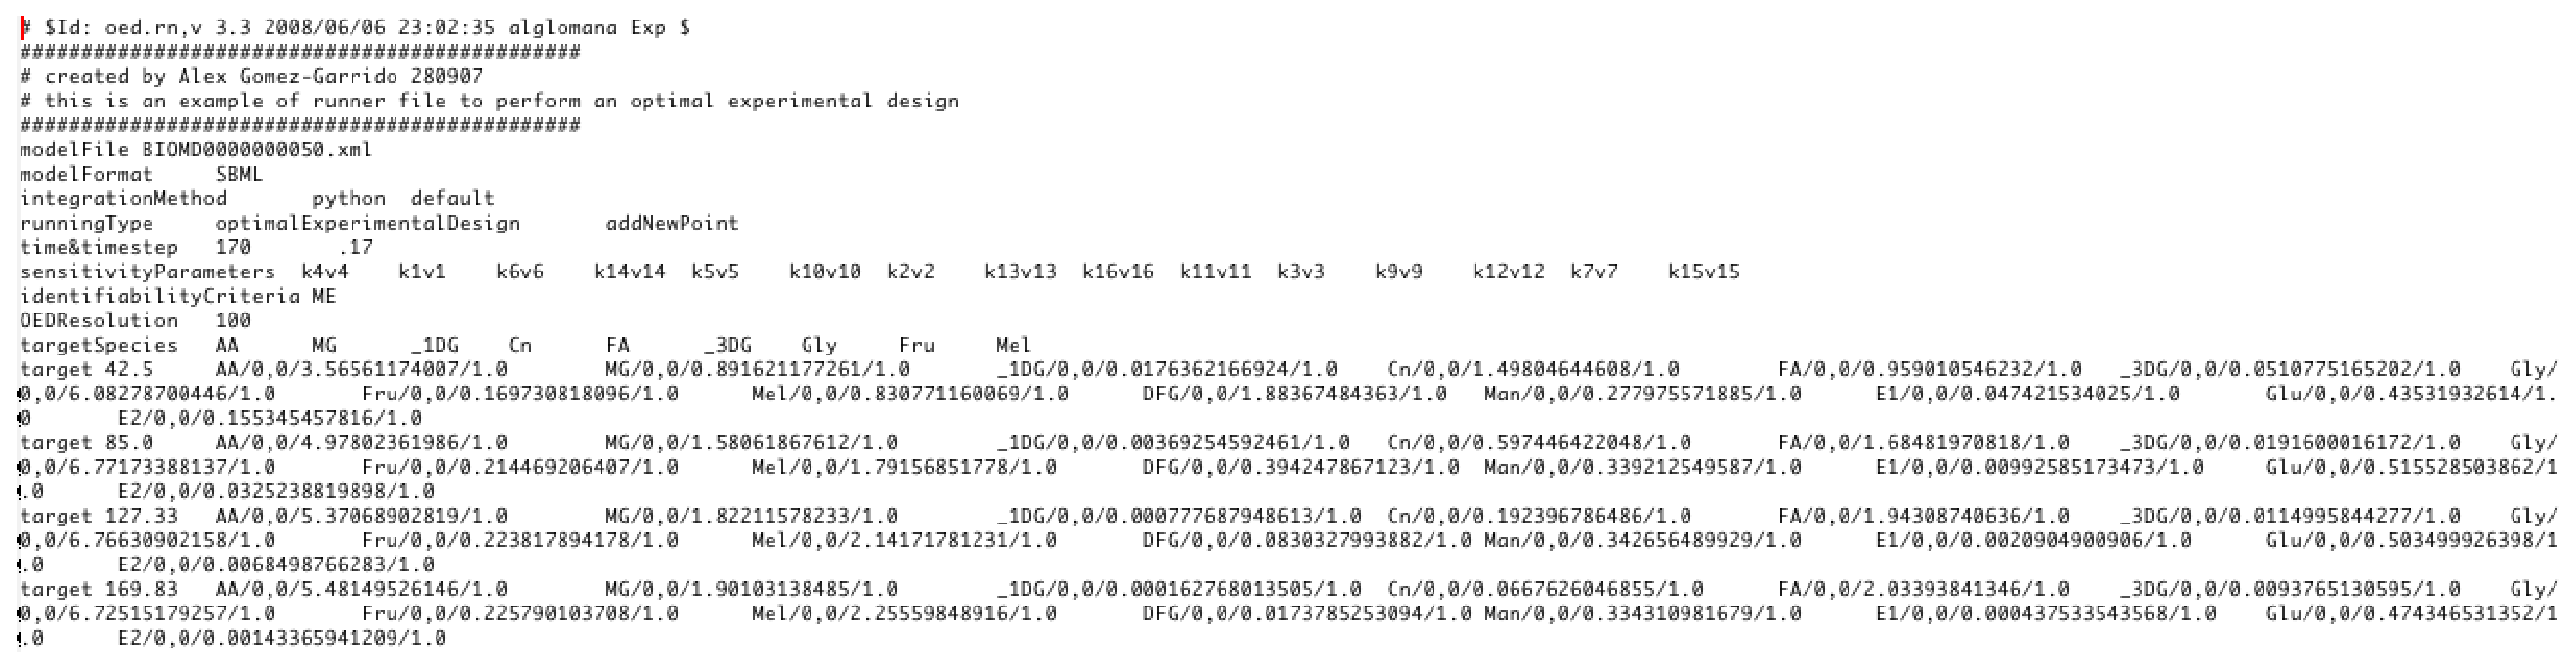
\includegraphics[scale=.5]{figures/oedRunner.eps}
      \caption{
        Snapshot of an example of \emph{runner} file for running an optimal experimental design protocol.
      }
      \label{oedRunner}
    \end{center}
  \end{figure}
  Apart from the \texttt{Kinetic\_modelling\_of\_Amadori\_degradation.out} and \\ \texttt{Kinetic\_modelling\_of\_Amadori\_degradation.ps} files described in Section \ref{simulation}, we have the following files specific of the OED analysis:
  \begin{itemize}
  \item \texttt{Kinetic\_modelling\_of\_Amadori\_degradation.oed.txt}:
    This is a text file where the most optimal values are stored.
    For each required criteria the best temporal point for each selected model species is saved.
  \item \texttt{Kinetic\_modelling\_of\_Amadori\_degradation.oed.}\textit{criteria}\texttt{.ps}:
    For each OED criteria a postscript figure is created showing the value of the corresponding criteria for each selected node and time.
    Blue colours show anticorrelation and red colour positive correlation.
    The intensity of the color is relative to the diagonal of the matrix.
  \end{itemize}
  \section{Tutorial}
  % information about the non dimention affectors should be included. The example should change.
  Mainly all the work of \texttt{ByoDyn} will be done from a terminal.
  A terminal is a tool to interact with the computer using commands.
  Locate the terminal on your operating system and launch it.
  All the text in \texttt{text font} corresponds to the commands you type on the terminal.
   First obtain the exercises from the directory where you installed \texttt{ByoDyn} and copy them into your home (or any other if you prefer) to start working:
   \begin{center}
     \texttt{cp -r \$BYODYN\_PATH/examples/tutorialExercises .}
   \end{center}
   If nothing happens, everything went well.
   Now you can go to the new created directory.
   To do that type the following.
  \begin{center}
    \texttt{cd tutorialExercises}
  \end{center}
  and check what is in there:
  \begin{center}
    \texttt{ls}
  \end{center}
  Three directories will appear containing computational  models of
  metabolism and gene regulation we will study. The first two models are
  publicly available at the \emph{BioModels Database} \url{http://www.ebi.ac.uk/biomodels/} and are in SBML format. SBML (Systems Biology Markup Language) is \textit{de facto} format for computational models.
  More than 90 software tools support it and an active community is behind it \url{http://sbml.org/index.psp}.
  These  models, involving gene regulation and metabolism, based on uni-cellular systems.
  The last one is the result of a multidisciplinary collaboration and simulates the early patterning and neural specification during early inner ear development. 
  In this often, we aim at studying gene regulation in a multicellular environment to understand pattern formation.
  \subsection{\textit{Amadori} Model}
  First change to the directory where the model and the options files for \texttt{ByoDyn} are:
  \begin{center}
    \texttt{cd amadori}\\
    \texttt{ls}
  \end{center}
  Among the different files, the file Amadori.xml contains the model description in SBML format.
  It is number 50 of the BioModels database ninth release.
  In addition, files with the .rn extension are the runner files for \texttt{ByoDyn} where the different tasks we want the program to do are specified.
  \subsubsection{Biological Background}
  This model accounts for sugar metabolism.
  Thermal decomposition of N-(1-deoxy--fructos-1-yl)-glycine (DFG) is a complicate kinetic pathway involving important metabolites as acetic acid, formic acid, glucose, fructose or mannose among others.
  From the metabolic network (please check Scheme 1 of \cite{martins03}) a kinetic model has been proposed in \citep{martins03}.
  The model leads to the following set of equations\footnote{the above set of equations were extracted by \texttt{ByoDyn} from the SBML file directly in the \texttt{.tex} format file \texttt{Kinetic\_modelling\_of\_Amadori\_degradation.tex} in the output directory}.
  \begin{center}
    \textbf{Kinetic laws:}
\tiny
\begin{eqnarray}
v12 & = &  k12*Man \\\nonumber & & \\
v13 & = &  k13*Glu \\\nonumber & & \\
v10 & = &  k10*E1 \\\nonumber & & \\
v11 & = &  k11*E1 \\\nonumber & & \\
v16 & = &  k16*E2 \\\nonumber & & \\
v14 & = &  k14*Cn*Gly \\\nonumber & & \\
v15 & = &  k15*Cn \\\nonumber & & \\
v1 & = &  k1*DFG \\\nonumber & & \\
v2 & = &  k2*DFG \\\nonumber & & \\
v3 & = &  k3*DFG \\\nonumber & & \\
v4 & = &  k4*E1 \\\nonumber & & \\
v5 & = &  k5*\_3DG \\\nonumber & & \\
v6 & = &  k6*\_3DG \\\nonumber & & \\
v7 & = &  k7*E2 \\\nonumber & & \\
v8 & = &  k8*\_1DG \\\nonumber & & \\
v9 & = &  k9*\_1DG \\\nonumber & & \\\nonumber
\end{eqnarray}
\normalsize
\textbf{ODEs:}
\tiny
\begin{eqnarray}
\frac{\mathrm{d}[DFG]_{i}}{\mathrm{d}t} & = & - v2- v3- v1 \\\nonumber & & \\
\frac{\mathrm{d}[E1]_{i}}{\mathrm{d}t} & = & + v1- v10- v4- v11 \\\nonumber & & \\
\frac{\mathrm{d}[E2]_{i}}{\mathrm{d}t} & = & - v7- v16+ v2 \\\nonumber & & \\
\frac{\mathrm{d}[Cn]_{i}}{\mathrm{d}t} & = & + v3- v14- v15+ v5+ v8 \\\nonumber & & \\
\frac{\mathrm{d}[Gly]_{i}}{\mathrm{d}t} & = & - v14+ v10+ v11+ v4+ v7+ v3+ v16 \\\nonumber & & \\
\frac{\mathrm{d}[\_3DG]_{i}}{\mathrm{d}t} & = & + v13- v5- v6+ v4 \\\nonumber & & \\
\frac{\mathrm{d}[FA]_{i}}{\mathrm{d}t} & = & + v6+ v15 \\\nonumber & & \\
\frac{\mathrm{d}[\_1DG]_{i}}{\mathrm{d}t} & = & - v8+ v7- v9 \\\nonumber & & \\
\frac{\mathrm{d}[AA]_{i}}{\mathrm{d}t} & = & + v9+ v15 \\\nonumber & & \\
\frac{\mathrm{d}[Man]_{i}}{\mathrm{d}t} & = & + v10- v12 \\\nonumber & & \\
\frac{\mathrm{d}[Glu]_{i}}{\mathrm{d}t} & = & + v11+ v12- v13 \\\nonumber & & \\
\frac{\mathrm{d}[MG]_{i}}{\mathrm{d}t} & = & + v15 \\\nonumber & & \\
\frac{\mathrm{d}[Mel]_{i}}{\mathrm{d}t} & = & + v14 \\\nonumber & & \\
\frac{\mathrm{d}[Fru]_{i}}{\mathrm{d}t} & = & + v16 \\\nonumber & & \\\nonumber
\end{eqnarray}

  \end{center}
  The study of the system computationally can give insights of the network parameters and reaction mechanisms.
  \subsubsection{Simulation}
  We will call \texttt{ByoDyn} with the file \texttt{simulation.rn} as argument. 
  In this file all the options for \texttt{ByoDyn} in order to run appropriately a simulation are stored.
  The default name of the option name for the output directory (\texttt{output}) can be changed to whatever other name by using the \texttt{-o} option as in:
  \begin{center}
    \texttt{byodyn -o simulation simulation.rn}
  \end{center}
  The result of the simulation is the calculation of the concentration of the reacting nodes along time.
  You can see the graph by making use of your preferred postscript viewer. For example:
  \begin{center}
    \texttt{ggv simulation/Kinetic\_modelling\_of\_Amadori\_degradation.ps\&}
  \end{center}
  DFG is degraded giving raise of a variety of products, mainly glycine (Gly) and acetic acid (AA).
  Please have a look to Figure \ref{amadoriSimulation.eps}.
  \begin{figure}
    \begin{center}
      \rotatebox{270}{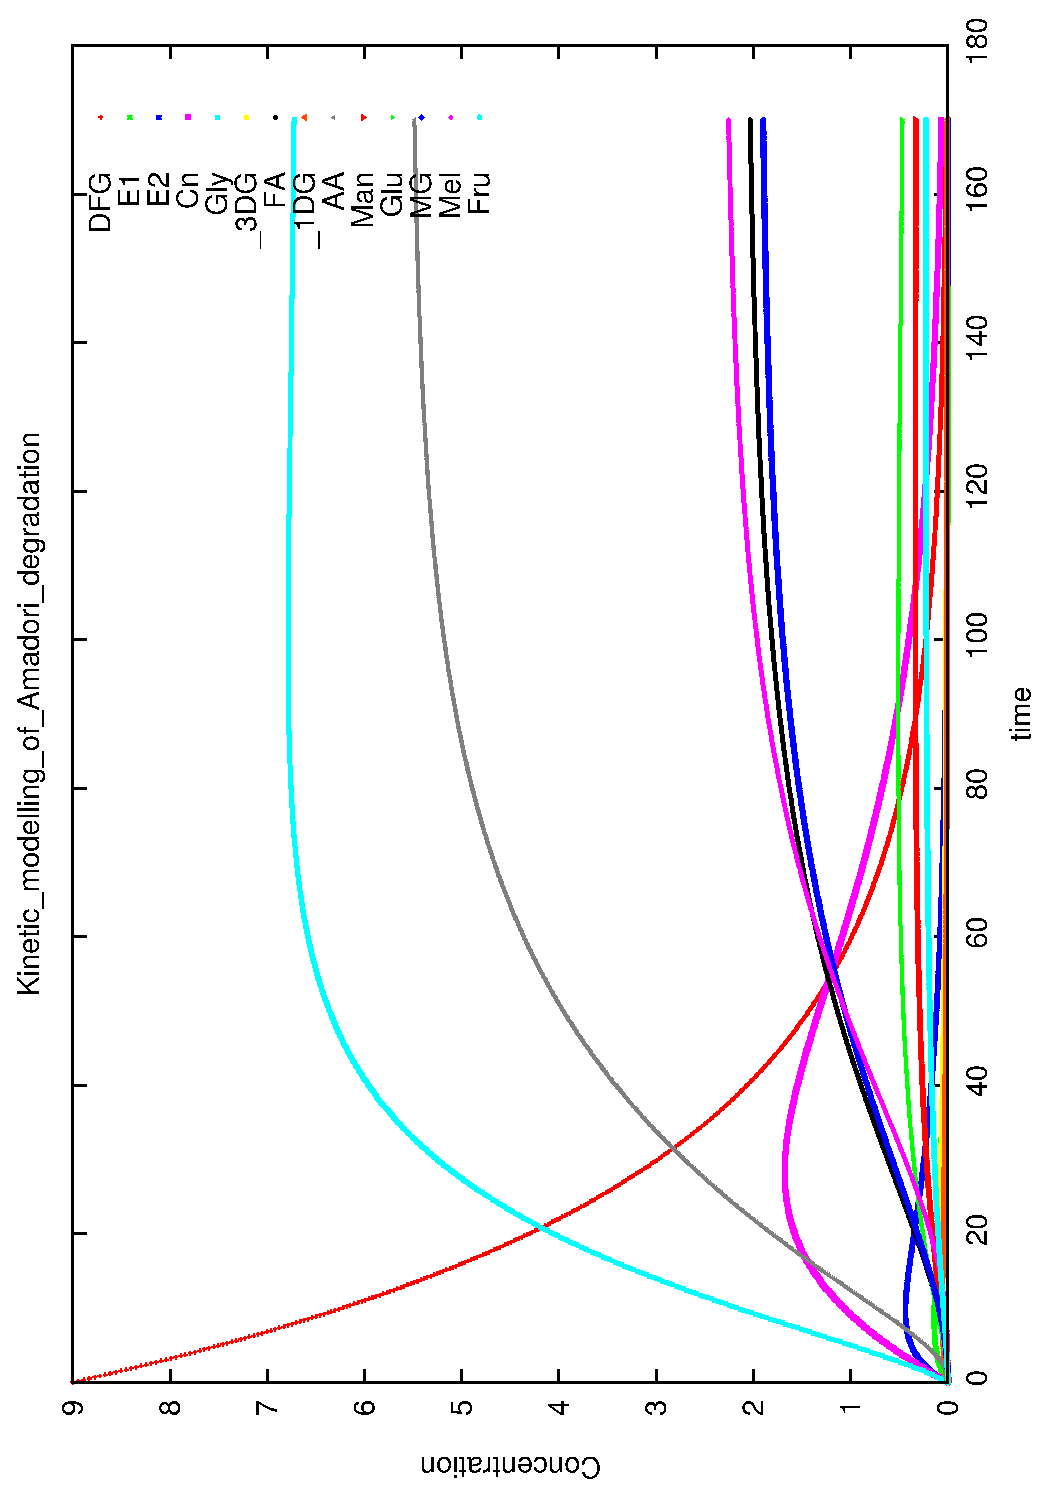
\includegraphics[scale=.5]{figures/amadori.eps}}
      \caption{Numerical trajectories of the simulation the Amadori simulation.}\label{amadoriSimulation.eps}
    \end{center}
  \end{figure} 
  \subsubsection{Sensitivity Analysis}
  Sensitivity analysis is a technique very informative to understand which is the key step on a reaction pathway.
  It is calculated as the change on the concentrations of a system while varying a parameter.
  Type the following for the study:
  \begin{center}
    \texttt{byodyn -o sensitivity sensitivity.rn}
  \end{center}
  See the results at:
  \begin{center}
    \scriptsize{\texttt{ggv sensitivity/Kinetic\_modelling\_of\_Amadori\_degradation.sens.global.timeCourse.ps}}
  \end{center}
  You will see the same results of Figure \ref{amadoriSensitivity}.
  \begin{figure}[!h]
    \begin{center}
      \rotatebox{270}{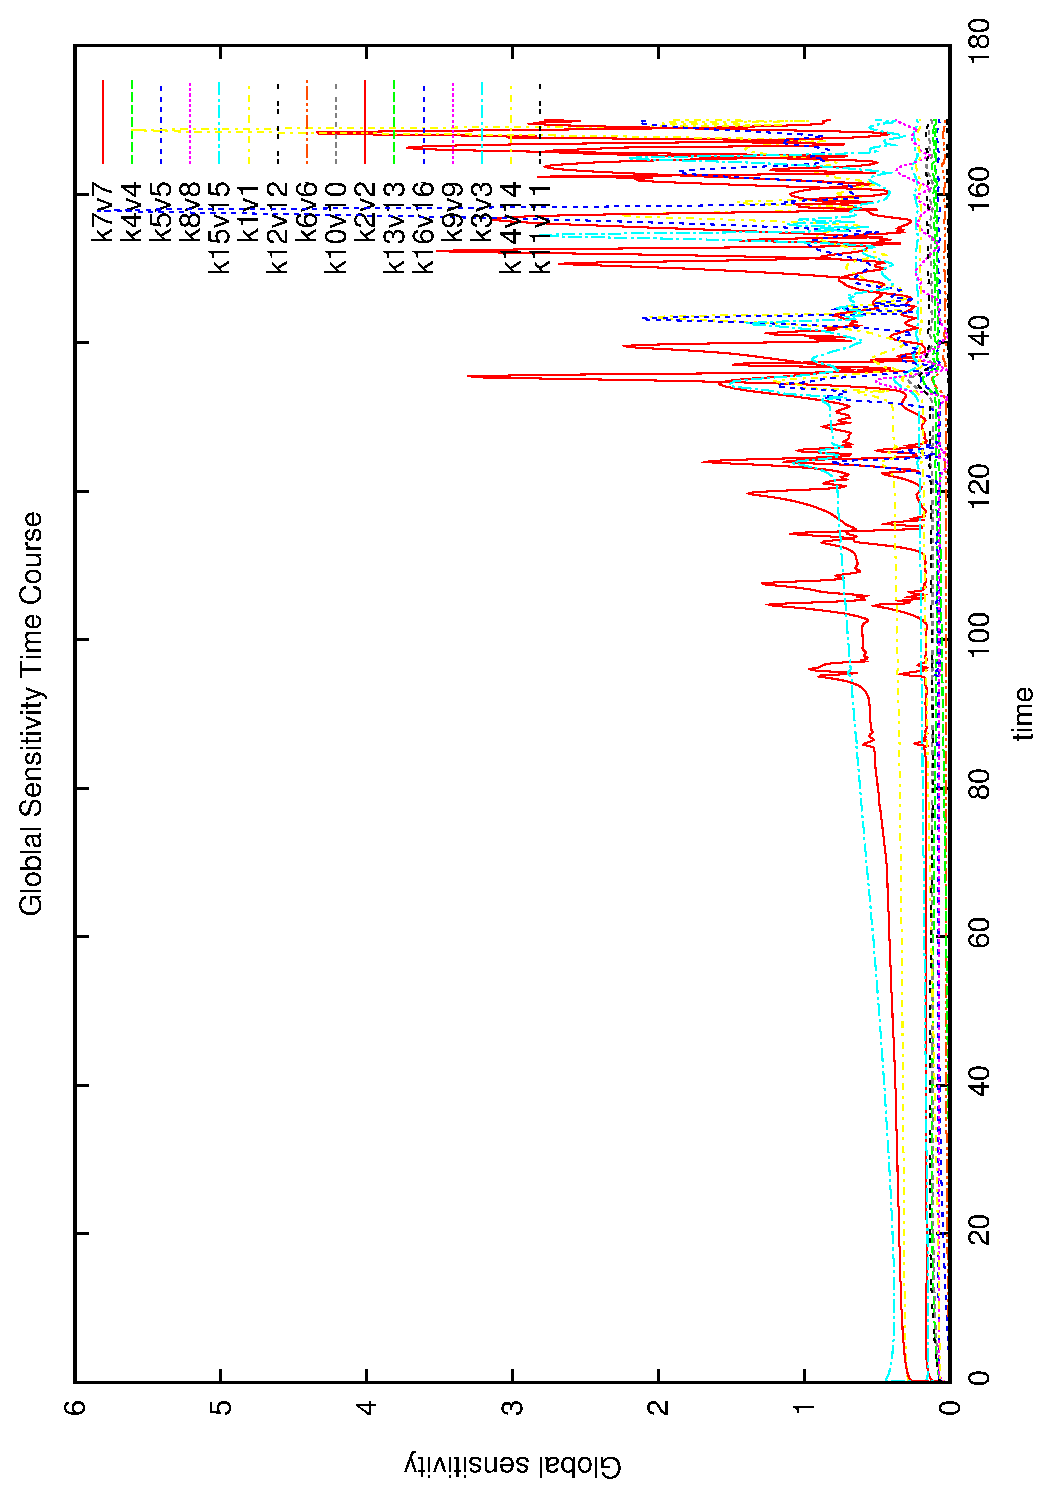
\includegraphics[scale=.5]{figures/amadoriSensitivity.eps}}
      \caption{Time course global sensitivity of the nodes of the Amadori model.}\label{amadoriSensitivity}
    \end{center}
  \end{figure}
  It is not very clear which parameter is the most sensitive in the model.
  We can have a better clue accessing the figure showing the matrix of sensitivities of nodes/parameters:
  \begin{center}
    \footnotesize{\texttt{ggv sensitivity/Kinetic\_modelling\_of\_Amadori\_degradation.sens.relative.ps}}
  \end{center}
  As you can see in Figure \ref{amadoriSensitivityMatrix}, the parameters with highest sensitivity are $k_2$, $k_1$. 
  \begin{figure}[!h]
    \begin{center}
      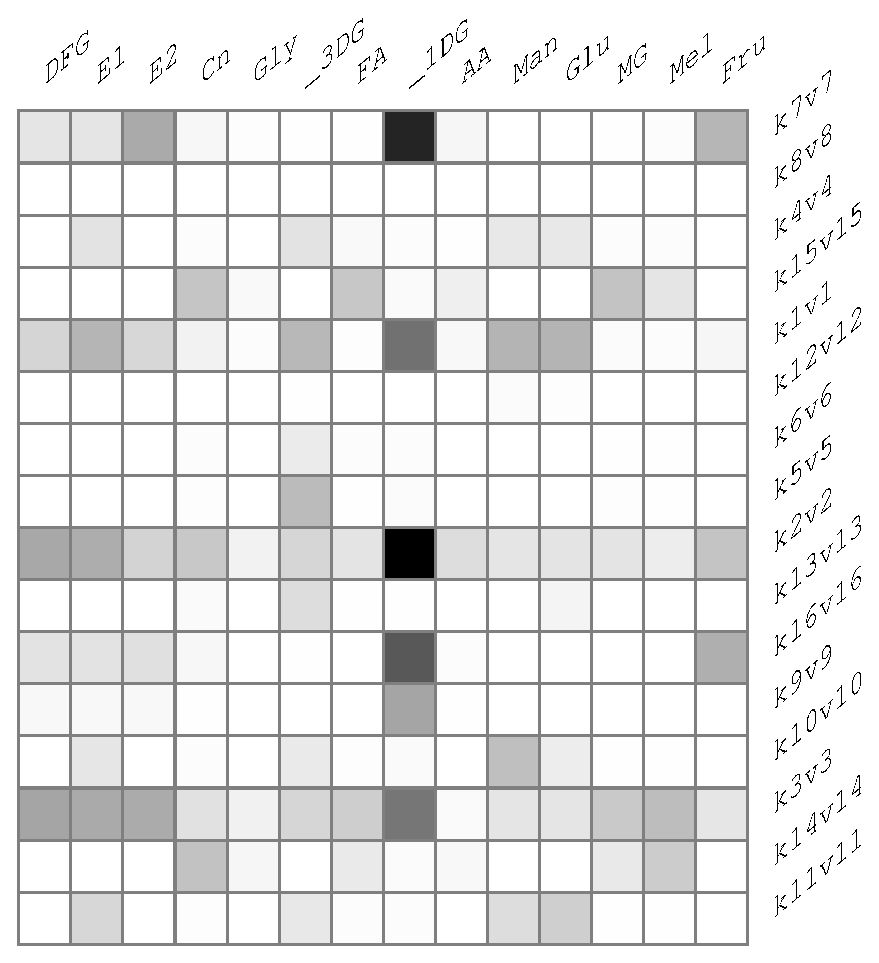
\includegraphics[scale=.5]{figures/amadoriSensitivityMatrix.eps}
      \caption{Relative sensitivity of the nodes with respect to the parameters of the Amadori model.}\label{amadoriSensitivityMatrix}
    \end{center}
  \end{figure}
  These constants regulate the degradation of DFG as seen in Equations 8, 9 and 17.
  Indeed, the degradation of this compound is known to be the trigger of the complete metabolic network.
  \subsubsection{Optimisation}
  The set of the parameters (degradation constants, binding constants, formation constants, etc.)  of this model are the following:
  \begin{center}
    \footnotesize{\texttt{cat simulation/Kinetic\_modelling\_of\_Amadori\_degradation.description.txt}}
  \end{center}
  Now, we can use optimisation techniques to infer the nominal values using a temporal experimental data set.
  Type the following for the optimisation:
  \begin{center}
    \texttt{byodyn -o optimisation optimisation.rn\&}
  \end{center}
  Optimisation techniques are computationally expensive.
  Specially global methods that commonly are based on stochastic variables.
  In this case the optimisation will run in the order of minutes.
  In the meantime let's have a look to the experimental data we are using:
  \begin{center}
    \texttt{emacs optimisation.rn}
  \end{center}
  Check the fitness function that represents a distance between the experimental data and the simulated results.
  \begin{equation}\label{eq:distance}
    F(\mathbf{p}) = \frac{1}{T_k}
    \sum_{i=1}^{T_k} 
    \frac
	{\left(y_{i}^{\mathrm{obs}} - y_{i}^{\mathrm{calc}}(\mathbf{p})\right)^2}
	{\sigma_i}
  \end{equation}
  Because the number of parameters is quite large, the final fitness function value for most of you will be around $10^{-3}$. 
  Are the optimal parameters close to the nominal ones?
  Could you explain what happened?
  If you are lucky the final value of your fitness function will be around $10^{-15}$. 
  Which are the values of the parameters?
  What happened instead?
  Could you compare the situation with the optimisation in Section \ref{optimisationSection}?
  If you would like to find the nominal values for all the parameters, change the optimisation method, instead of \texttt{hybridTwoPhases} set it as \texttt{hybridOnePhase} and the convergence will occur.
  In our tests, it took less than 8 minutes the \texttt{hybridTwoPhases} optimisation and several hours for the \texttt{hybridOnePhase} calibration on a 1.83 GHz Intel Core Duo.
  \subsection{\textit{Repressilator} Model}
  \subsubsection{Biological Background}
  The model is composed of three genes and their genetic products.
  Each of the gene products inhibits the transcription of the other one (Figure \ref{repressilator}).
  This system was artificially engineered on bacteria organism as a proposed oscillator.
  \begin{figure}[!t]
    \begin{center}
      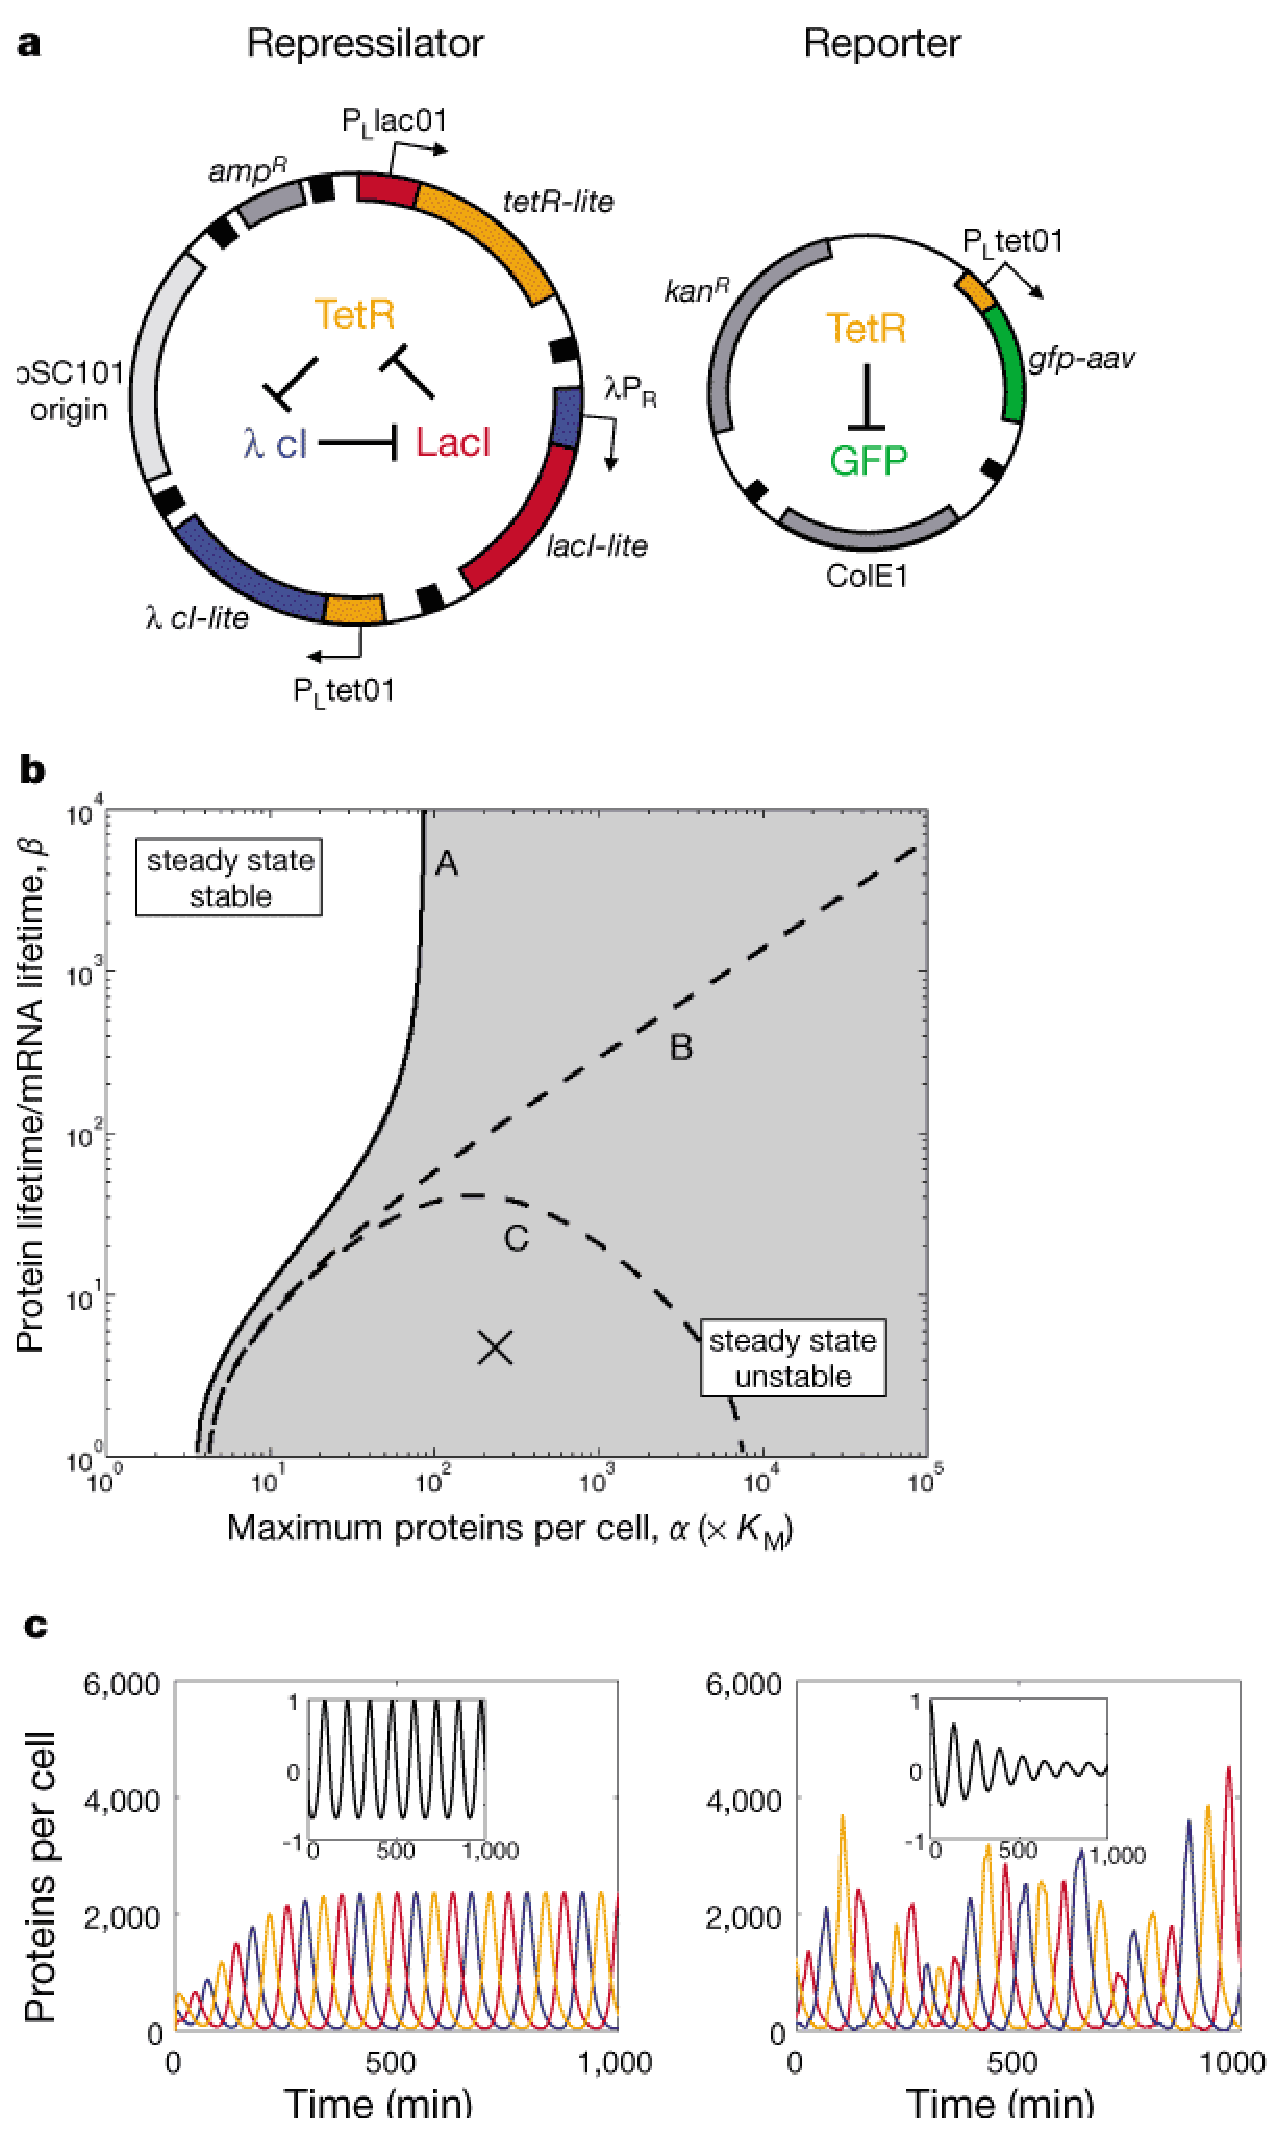
\includegraphics[bb=5 670 310 980,clip,width=0.49\linewidth]{figures/plasmid.eps}
      \caption{Figure obtained from \cite{elowitz00}. The proposed network was built on a plasmid.\label{repressilator}}
    \end{center}
  \end{figure} 
  More information can be found at the original article \citep{elowitz00}.
  \subsubsection{Simulation}
  First of all change to the corresponding directory:
  \begin{center}
    \texttt{cd ../repressilator}
  \end{center}
  And execute the corresponding command:
  \begin{center}
    \texttt{byodyn -o simulation simulation.rn}
   \end{center}
   As you can see at the simulation results, 
   \begin{center}
     \texttt{ggv simulation/repressilator.ps}
   \end{center}
   the network behaves as an oscillator.
   These parameters account for the phenotype that has been checked experimentally.
   Now, we can change the value of the parameters and observe that the dynamics of the system differ.
   The parameters used for the former simulation were the original ones of the SBML as you can see in the file:
   \begin{center}
     \texttt{cat simulation/repressilator.description.txt}
   \end{center}
   In order to change the value of the parameter of the model, you have to edit the file \texttt{simulation.rn} file adding the following line:
   \begin{center}
     \texttt{parameters   name\_of\_parameter=value  ...}
   \end{center}
   We suggest to use \texttt{Emacs} as editor:
   \begin{center}
     \texttt{emacs simulation.rn}
   \end{center}
   Let's vary the parameter $n$ by adding the following line: 
   \begin{center}
     \texttt{parameter	alpha=5			beta=100}
   \end{center}
   and run the simulation again.
   Can you explain the differences on the dynamical behavior from the last simulation?
   We suggest you to have a look to the system of ODEs (Ordinary Differential Equations):
   \begin{center}
     \texttt{cd simulation}\\
     \texttt{pdflatex repressilator.tex}\\
     \texttt{ggv simulation.pdf}
   \end{center}
   and Figure 1b of the \cite{elowitz00} publication.
  \subsubsection{Sensitivity Analysis}
  Perform the sensitivity analysis:
  \begin{center}
    \texttt{byodyn -o sensitivity sensitivity.rn}
  \end{center}
  As you can see the exponent $n$ is the most sensitive parameter of the network.
  Also the dynamics are greatly affected by the half live of the mRNA.
  \subsubsection{Optimisation} \label{repressilatorOptimisation}
  We will perform the optimisation of the two most sensitive parameters on a range of two orders of magnitude:
  \begin{center}
    \texttt{byodyn -o optimisation optimisation.rn}
  \end{center}
  The model calibration takes several minutes although the convergence is not achieved with fitness function values at the order of $10^{5}$.
  To gain further insights about why the optimisation was not successful, we studied the fitness function in the surroundings of the nominal values of the parameters in the next section.
  \subsubsection{Fitness Function Surfaces}
  We can build the fitness function surface running the \texttt{ByoDyn} option file \texttt{surface60.rn}.
  The resolution is largely poor to determine the relative size of the well of the global minimum therefore we ran the same option file but for a resolution of 500 points for each variable.
  The execution lasted for several hours on a single PC, approximately 16 hours of CPU for each 500 points resolution figure.
  \begin{figure}
    \begin{center}
      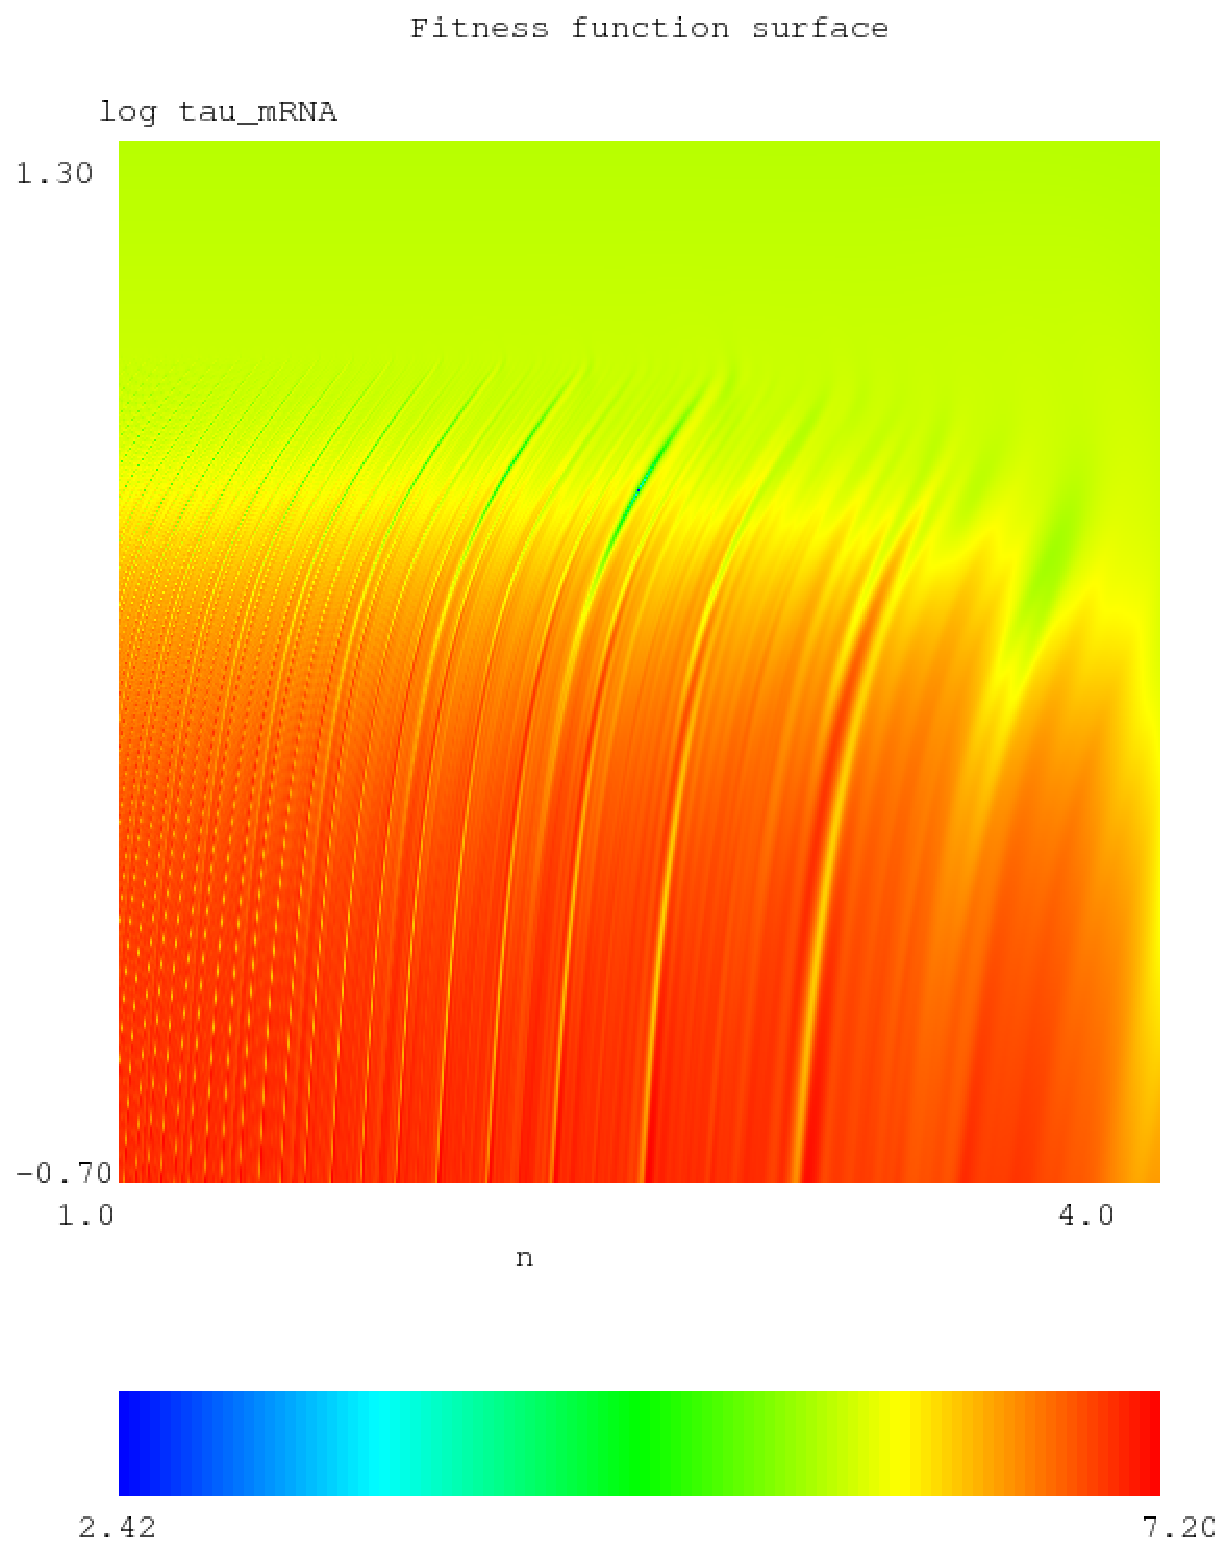
\includegraphics[scale=.75]{figures/60repressilator.eps}
      \caption{Fitness function surface of $n$ and $tau\_mRNA$ for the optimisation problem of section \ref{repressilatorOptimisation}.\label{amadori60}}
    \end{center}
  \end{figure}
  As it can be seen in Figure \ref{amadori60} the section of the well of the global minimum is so small that its finding is practically very difficult.
  An interesting study is the evolution of the fitness function in the surroundings of the global minimum well along the addition of new targeting data.
  The files \texttt{surface6.rn}, \texttt{surface60.rn}, \texttt{surface600.rn} and \texttt{surface6000.rn} were executed with a resolution of 500 points. 
  The computational cost was in the order of days for each surface on a Intel Core 2 Duo.
  Figure \ref{surfaceComparison} shows that adding experimental data points makes the surface smoother and the model calibration becomes much easier.
  \begin{figure}
    \begin{center}
      \begin{tabular}{cc}
        \multicolumn{1}{l}{\mbox{\bf a.}} & \multicolumn{1}{l}{\mbox{\bf b.}} \\
        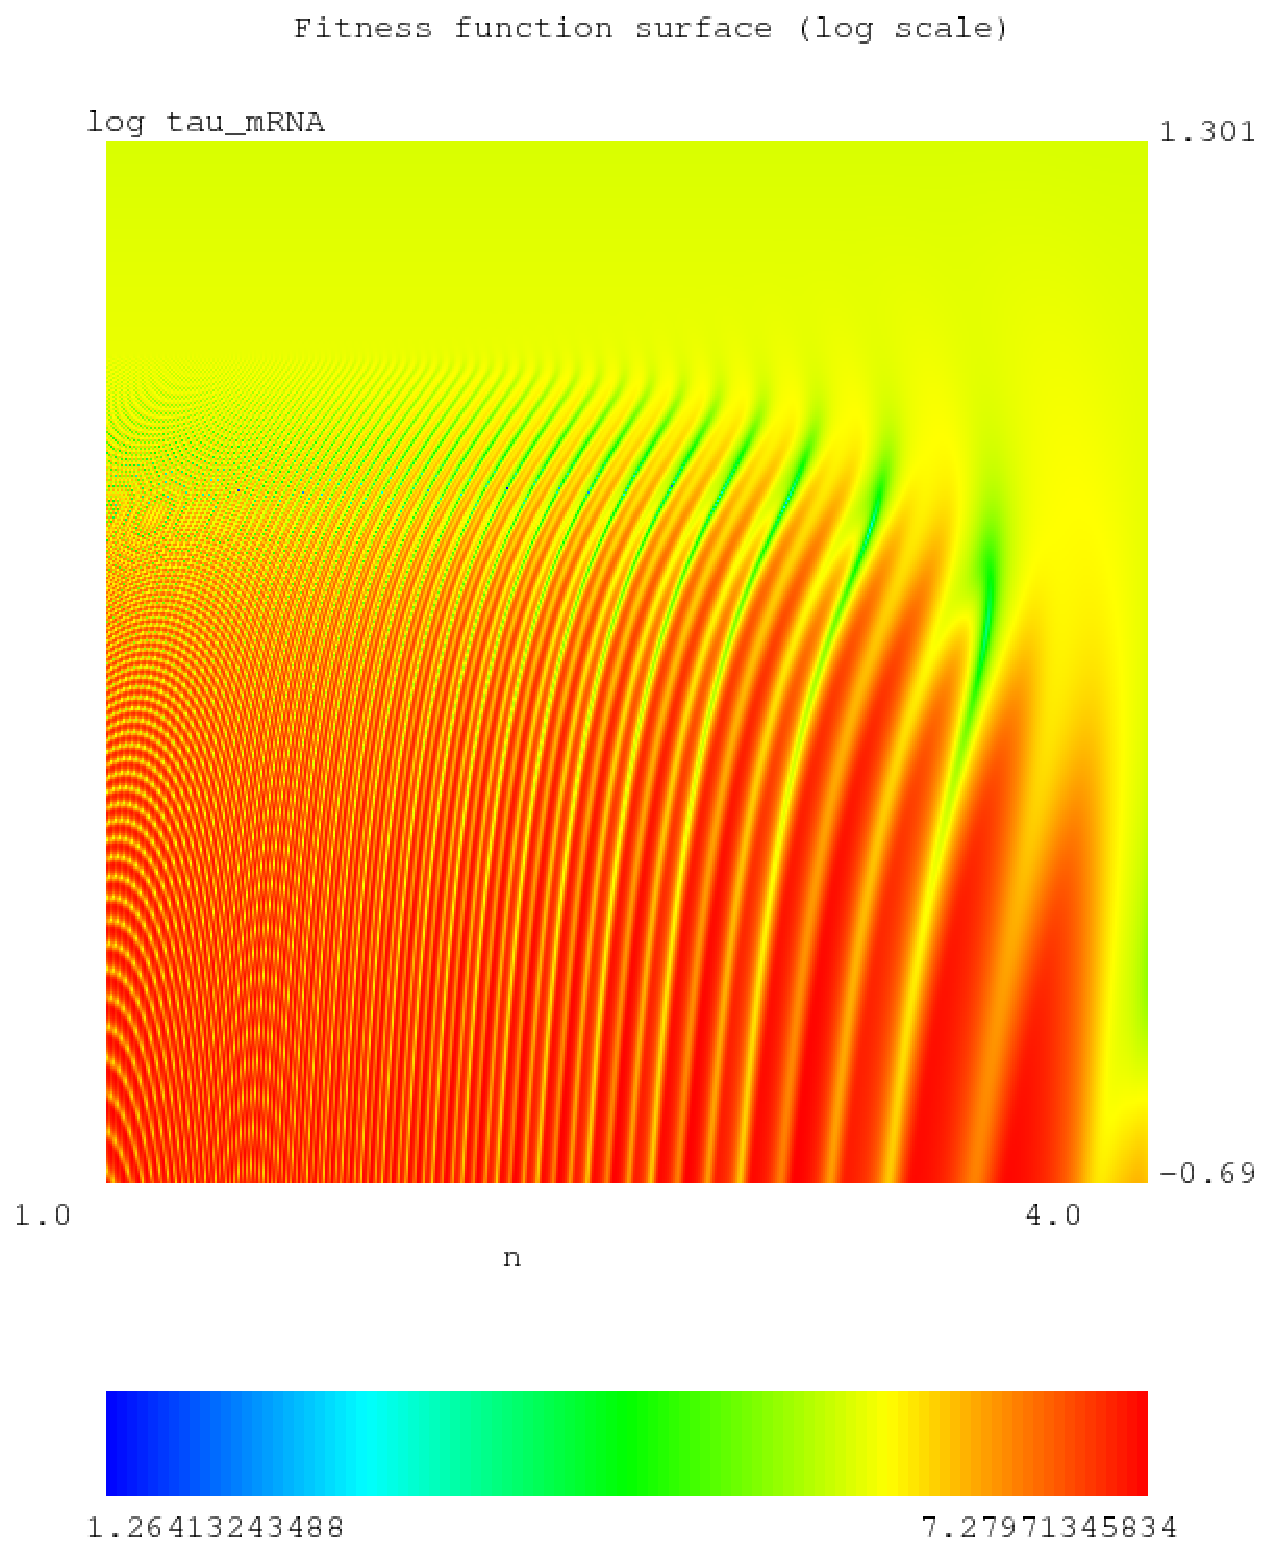
\includegraphics[bb=120 300 500 660,clip,width=.6\linewidth]{figures/6repressilator.eps}&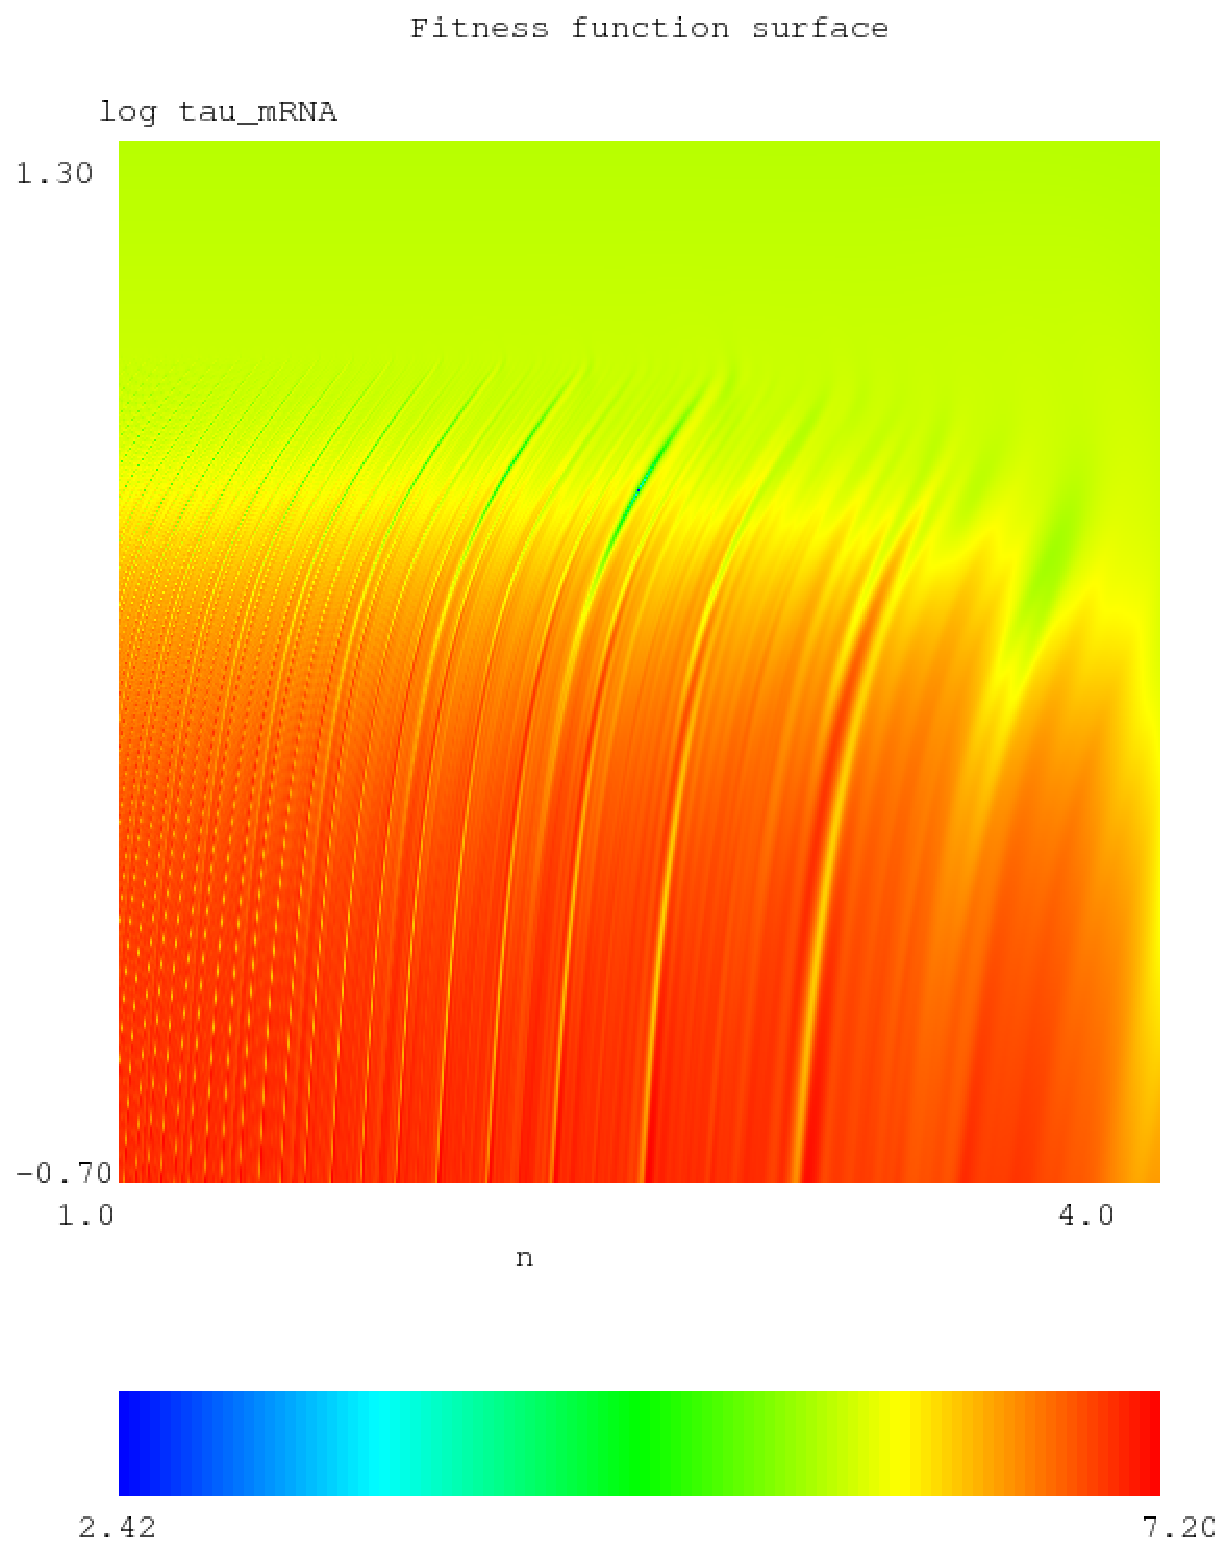
\includegraphics[bb=120 300 500 660,clip,width=.6\linewidth]{figures/60repressilator.eps}\\
        \multicolumn{1}{l}{\mbox{\bf c.}} & \multicolumn{1}{l}{\mbox{\bf d.}} \\
        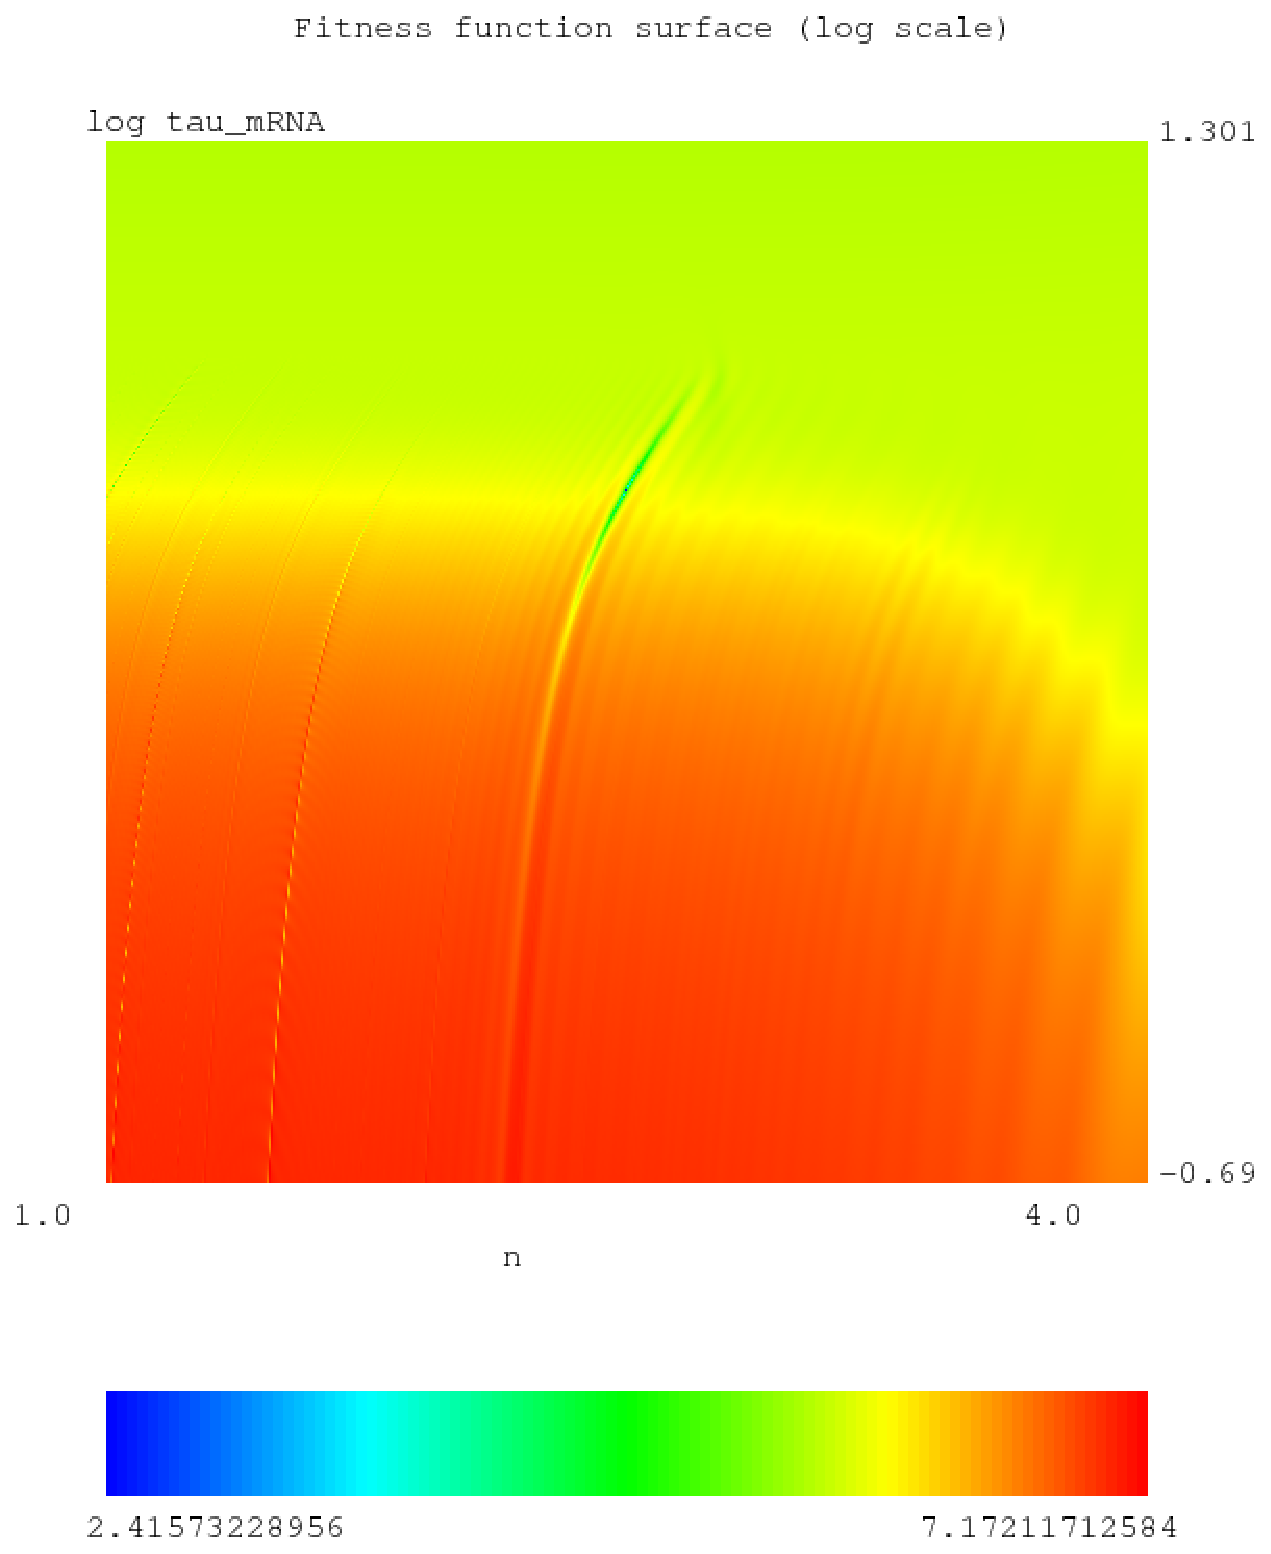
\includegraphics[bb=120 300 500 660,clip,width=.6\linewidth]{figures/600repressilator.eps}&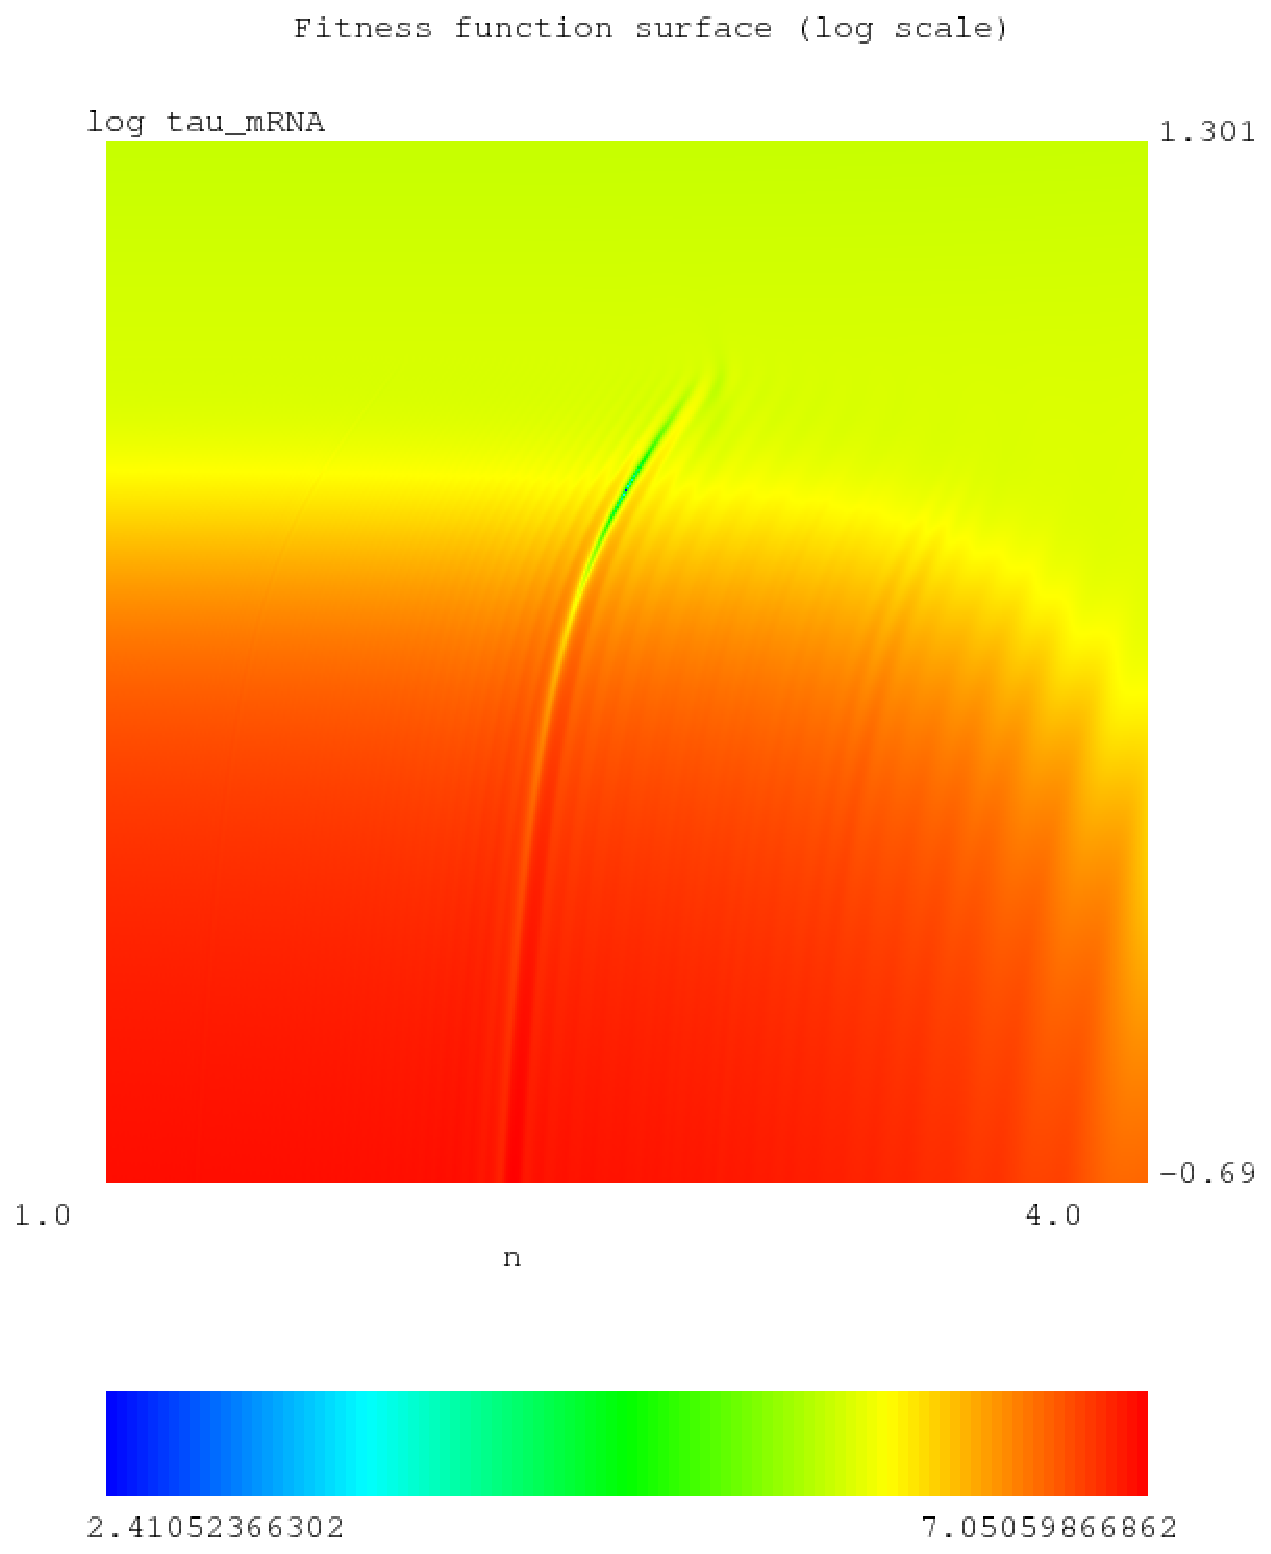
\includegraphics[bb=120 300 500 660,clip,width=.6\linewidth]{figures/6000repressilator.eps}\\
        \end{tabular}
      \caption{Fitness function surfaces for 6 ({\bf a.}), 60 ({\bf b.}), 600 ({\bf c.}) and 6000 ({\bf d.}) target points. 
        Note that the section of the global minimum well maintains its section but the number of local minima reduces considerably.
        \label{surfaceComparison}}
    \end{center}
  \end{figure}
  \subsection{\textit{Notch-Delta} Model}
  \subsubsection{Biological Background}
  The otic placode is a transitory structure that will give raise to the inner ear.
  During the its development cell fate is achieved by lateral inhibition and other biological pattern formation methods as boundary formation.
  Further information can be found at \citep{alsina04}.
  On the computational work we have focus on the lateral inhibition mechanism (Figure \ref{li}).
  \begin{figure}[!t]
    \begin{center}
      \includegraphics[scale=.5]{figures/li.eps}
      \caption{Lateral inhibition is based on the interactions of Notch and Delta.\label{li}}
    \end{center}
  \end{figure}
  \subsubsection{Simulation}
  Run the simulation as usual:
  \begin{center}
    \texttt{cd ../notch}\\
    \texttt{byodyn simulation5.rn} 
  \end{center}
  Check the results using again the graphical program \texttt{ggv},
  \begin{center}
    \texttt{ggv output/otic25cell.grid.ps}
  \end{center}
  as we show in Figure \ref{multicellular}.
  \begin{figure}
    \begin{center}
      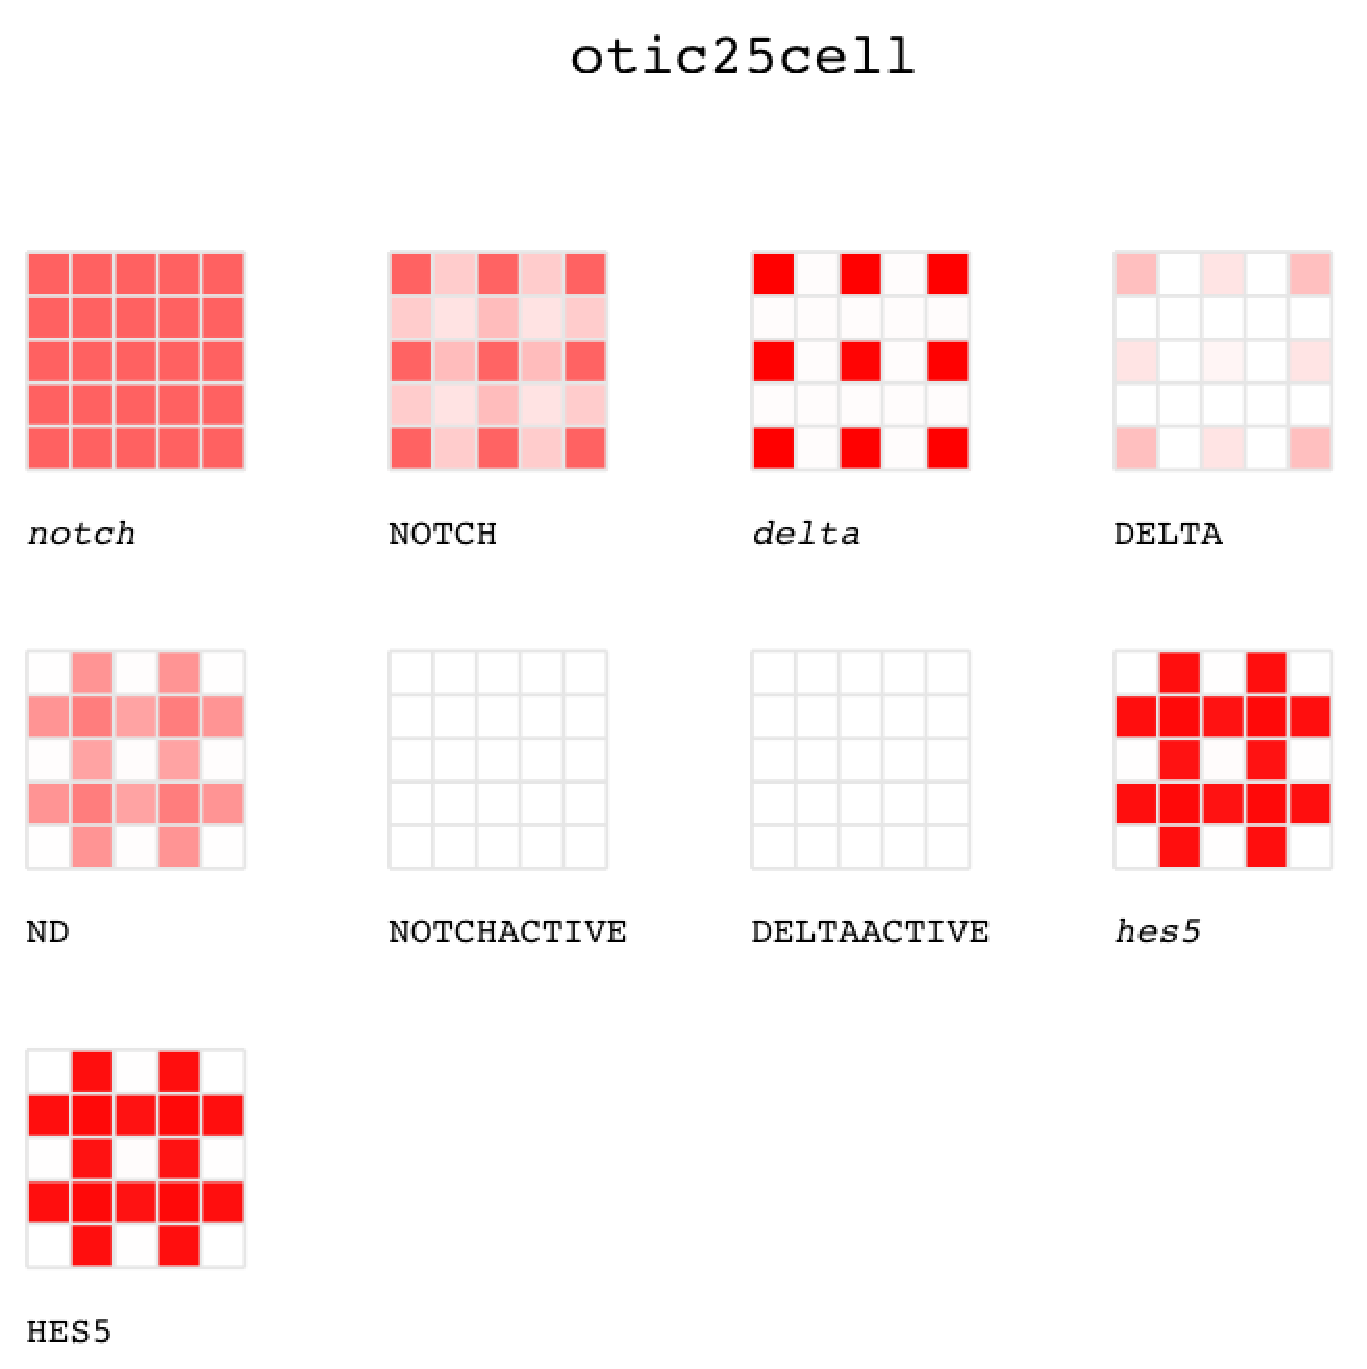
\includegraphics[scale=.5]{figures/multicellular.eps}
      \caption{Multicellular plot of a process of lateral inhibition on an epithelium of 25 cells.
        The figure represents the steady state of the trajectories of the system at time $t=3000$.
        \label{multicellular}}
    \end{center}
  \end{figure}
  You can also run the models of 2, 9 and 49 cell matrices.
  Simply note that it takes around 7 and 25 minutes the simulation of models containing 25 and 49 cells respectively on an Intel Core Duo 1,83 GHz.
  \bibliography{library.bib}
  \bibliographystyle{plainnat}
\end{document}
